\documentclass[aspectratio=169]{beamer}
\usepackage[utf8]{inputenc}
\usepackage[brazilian]{babel}
% Pacotes gráficos
\usepackage{svg}
\usepackage{epstopdf}
\usepackage{graphics}
\usepackage{media9}
\usepackage[export]{adjustbox}
\graphicspath{Fig}

% Pacotes matemáticos
\usepackage{icomma}
\usepackage{amsmath}
\usepackage{amssymb}
\usepackage{array}
\usepackage{arydshln}

% Tabelas
\usepackage{booktabs}

% Unidade de medida
\usepackage{siunitx}
\sisetup{output-decimal-marker={,},group-minimum-digits=4,abbreviations}
\sisetup{inter-unit-product=\ensuremath{{}\cdot{}}}

% Codigos
\usepackage{courier}
\usepackage{tcolorbox}
\tcbuselibrary{minted,breakable,xparse,skins}

\definecolor{turquesa}{rgb}{0,169,191}
\definecolor{bg}{gray}{0.95}
\DeclareTCBListing{mintedbox}{O{}m!O{}}{%
  breakable=true,
  listing engine=minted,
  listing only,
  minted language=#2,
  minted style=default,
  minted options={%
    linenos,
    gobble=0,
    breaklines=true,
    breakafter=,,
    fontsize=\small,
    numbersep=8pt,
    #1},
  boxsep=0pt,
  left skip=0pt,
  right skip=0pt,
  left=25pt,
  right=0pt,
  top=3pt,
  bottom=3pt,
  arc=5pt,
  leftrule=0pt,
  rightrule=0pt,
  bottomrule=2pt,
  toprule=2pt,
  colback=bg,
  colframe=orange!70,
  enhanced,
  overlay={%
    \begin{tcbclipinterior}
    \fill[orange!20!white] (frame.south west) rectangle ([xshift=20pt]frame.north west);
    \end{tcbclipinterior}},
  #3}

% Fonte
\usepackage{bookman} %font utopia imported

% Operadores matemáticos
\DeclareMathOperator{\sen}{sen}
\DeclareMathOperator{\Rot}{Rot}
\DeclareMathOperator{\Trans}{Trans}

% Tema
\useoutertheme{miniframes} % Alternatively: miniframes, infolines, split
\definecolor{UBCblue}{rgb}{0.04706, 0.13725, 0.26667} % UBC Blue (primary)
\usecolortheme[named=UBCblue]{structure}
\usetheme{Madrid}
\setbeamertemplate{page number in head/foot}{\makebox[5em][r]{\insertframenumber/\inserttotalframenumber}}
%\usecolortheme{default}
%\pgfminorversion=7

%------------------------------------------------------------
%This block of code defines the information to appear in the
%Title page
\title[Cinemática direta] %optional
{Método Clássico de Denavit-Hartenberg Aplicado ao KUKA LBR iiwa}

%\subtitle{A short story}

\author[] % (optional)
{A.~C.~Pereira\inst{1}, \and
B.~Bresolini\inst{1}, \and
F.~H.~N.~Resende\inst{1}, \and
I.~A.~Bastos\inst{1}, \and
K.~Geamonoud\inst{1}, \and
M.~O.~Coelho\inst{1}, \and
O.~G.~B.~de~O.~e~Oliveira\inst{1}, \and
T.~O.~Campagnani\inst{1}}


\institute[CEFET-MG] % (optional)
{
  \inst{1}%
  Graduandos em Eng. Mecatrônica\\
  Departamente de Eng. Mecatrônica, CEFET-MG
}

\date[Divinópolis, 2020] % (optional)
{Divinópolis, Setembro 2020}

%\logo{\includegraphics[height=1.5cm]{lion-logo.jpg}}

%End of title page configuration block
%------------------------------------------------------------



%------------------------------------------------------------
%The next block of commands puts the table of contents at the 
%beginning of each section and highlights the current section:

\AtBeginSection[]
{
  \begin{frame}
    \frametitle{Sumário}
    \tableofcontents[currentsection]
  \end{frame}
}
%------------------------------------------------------------

\pagenumbering{gobble}
\begin{document}

%The next statement creates the title page.
\frame{\titlepage}


%---------------------------------------------------------
%This block of code is for the table of contents after
%the title page
\begin{frame}
\frametitle{Sumário}
\tableofcontents
\end{frame}
%---------------------------------------------------------


\section{Apresentação}

%---------------------------------------------------------
{
\usebackgroundtemplate{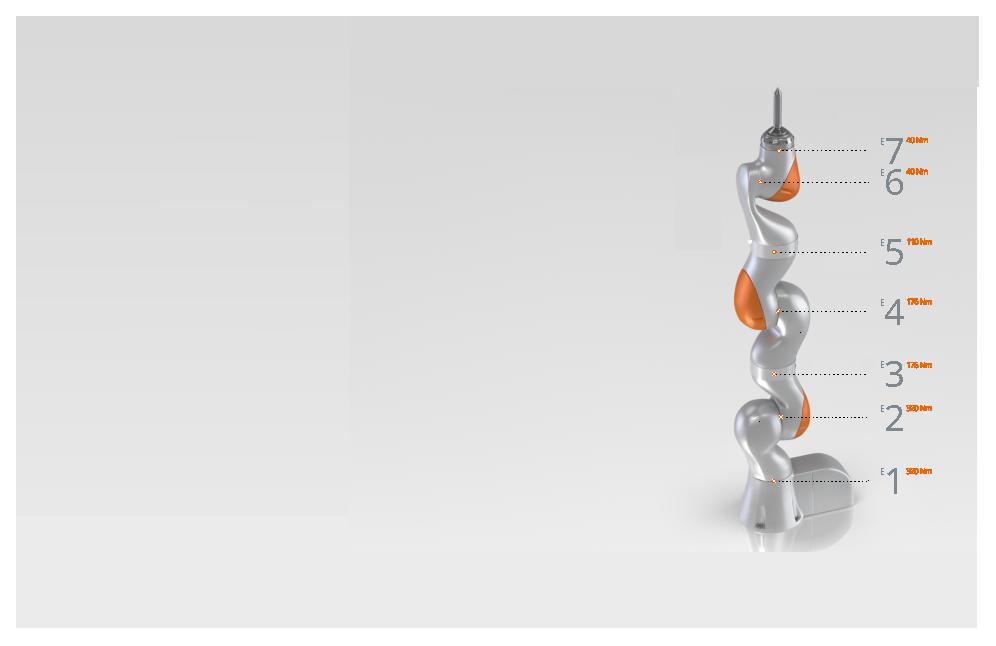
\includegraphics[width=\paperwidth]{Fig/Eixos.eps}}%

\begin{frame}{KUKA LBR iiwa}
\begin{minipage}[t]{0.6\textwidth}
O robô KUKA LBR iiwa é conhecido como novo antropomorfo e contém 7 graus de liberdade.

Existem dois padrões vendidos: LBR iiwa 7 800 e \alert{LBR iiwa 14 820}. O primeiro com carga efetiva de até 7 kg e o segundo com 14 kg.

\end{minipage}%
\end{frame}
}
\begin{frame}{KUKA LBR iiwa}
\begin{minipage}{0.45\textwidth}
\includemedia[width=0.98\textwidth,activate=pageopen,
passcontext,
transparent,
addresource=movie1.mp4,
flashvars={source=movie1.mp4}
]{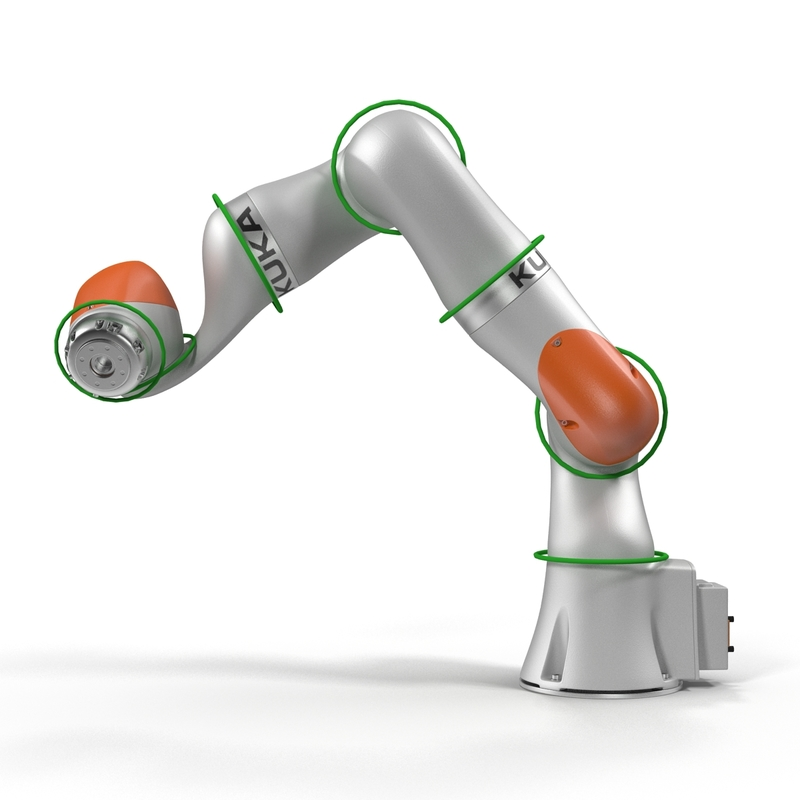
\includegraphics[width=0.55\textwidth]{Fig/01.jpg}}{VPlayer.swf}
\end{minipage}\hfill
\begin{minipage}{0.53\textwidth}
    Sua estrutura cinemática é do tipo esférica-rotacional-esférica (SRS) e seu volume de trabalho é uma esfera de 1,7 a 1,8 \si{m^3}.
\end{minipage}
\end{frame}

\section{Modelagem}

{
\usebackgroundtemplate{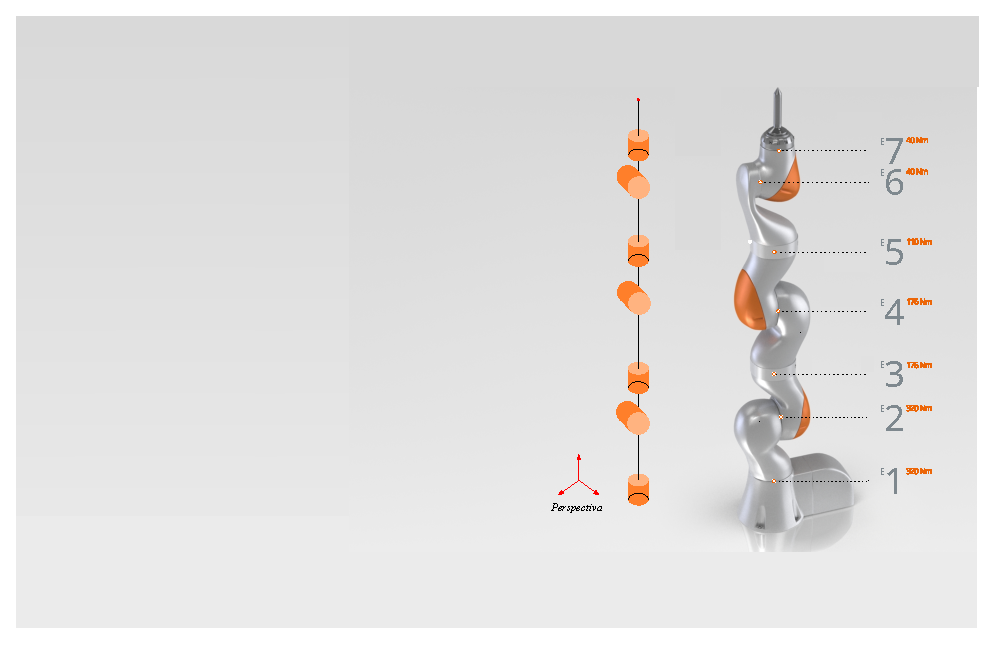
\includegraphics[width=\paperwidth]{Fig/Arames.eps}}%
\begin{frame}{Diagrama de arames}
    \begin{minipage}{0.5\textwidth}
        O primeiro passo para a apli\-cação do método clássico de Denavit-Hartenberg é desenhar o diagrama de arames para o manipulador robótico.
    \end{minipage}
\end{frame}
}
\begin{frame}{Atribuição de frames}
\begin{minipage}{0.7\textwidth}
    Inicialmente, deve-se atribuir os eixos $z_i$ nos eixos de atuação, para cada junta $i+1$, sendo $i = 0,\;1,\;2\dots,\;n-1$. A última junta é o \textbf{end-effector} ou o \textbf{tool frame} e, pode ser atribuído ao final.
\end{minipage}\hfill
\begin{minipage}{0.28\textwidth}
    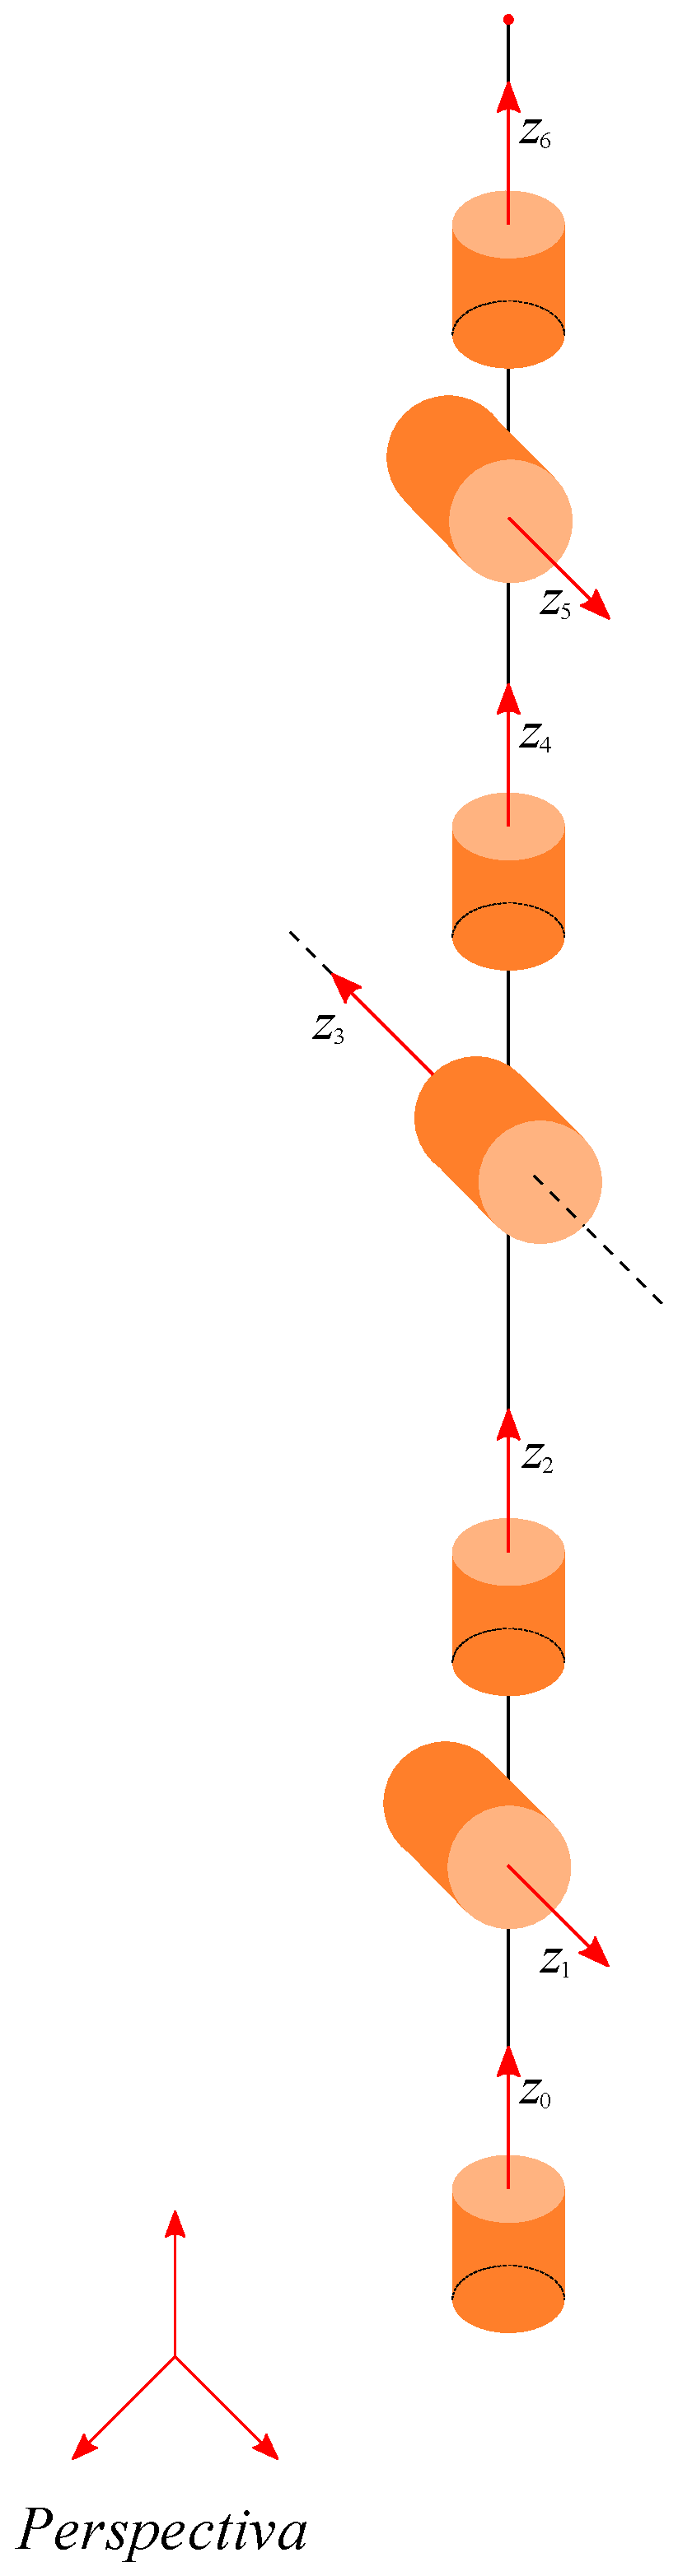
\includegraphics[width=0.45\textwidth]{Fig/z.eps}
\end{minipage}
\end{frame}


\begin{frame}{Atribuição de frames}
\begin{minipage}{0.58\textwidth}
    De acordo com SPONG, HUTCHINSON e VIDYASAGAR (2005, p. 74), se $z_{i-1}$ \alert{intercepta} $z_i$, $x_i$ é escolhido no plano normal formado por $z_i$ e $z_{i-1}$. O sentido positivo de $x_i$ é arbitrária e a origem $o_i$ pode ser atribuído no ponto de interseção de $z_i$ e $z_{i-1}$. Se isto for feito, o parâmetro $a_i$ será igual a 0.
\end{minipage}\hfill
\begin{minipage}{0.38\textwidth}
    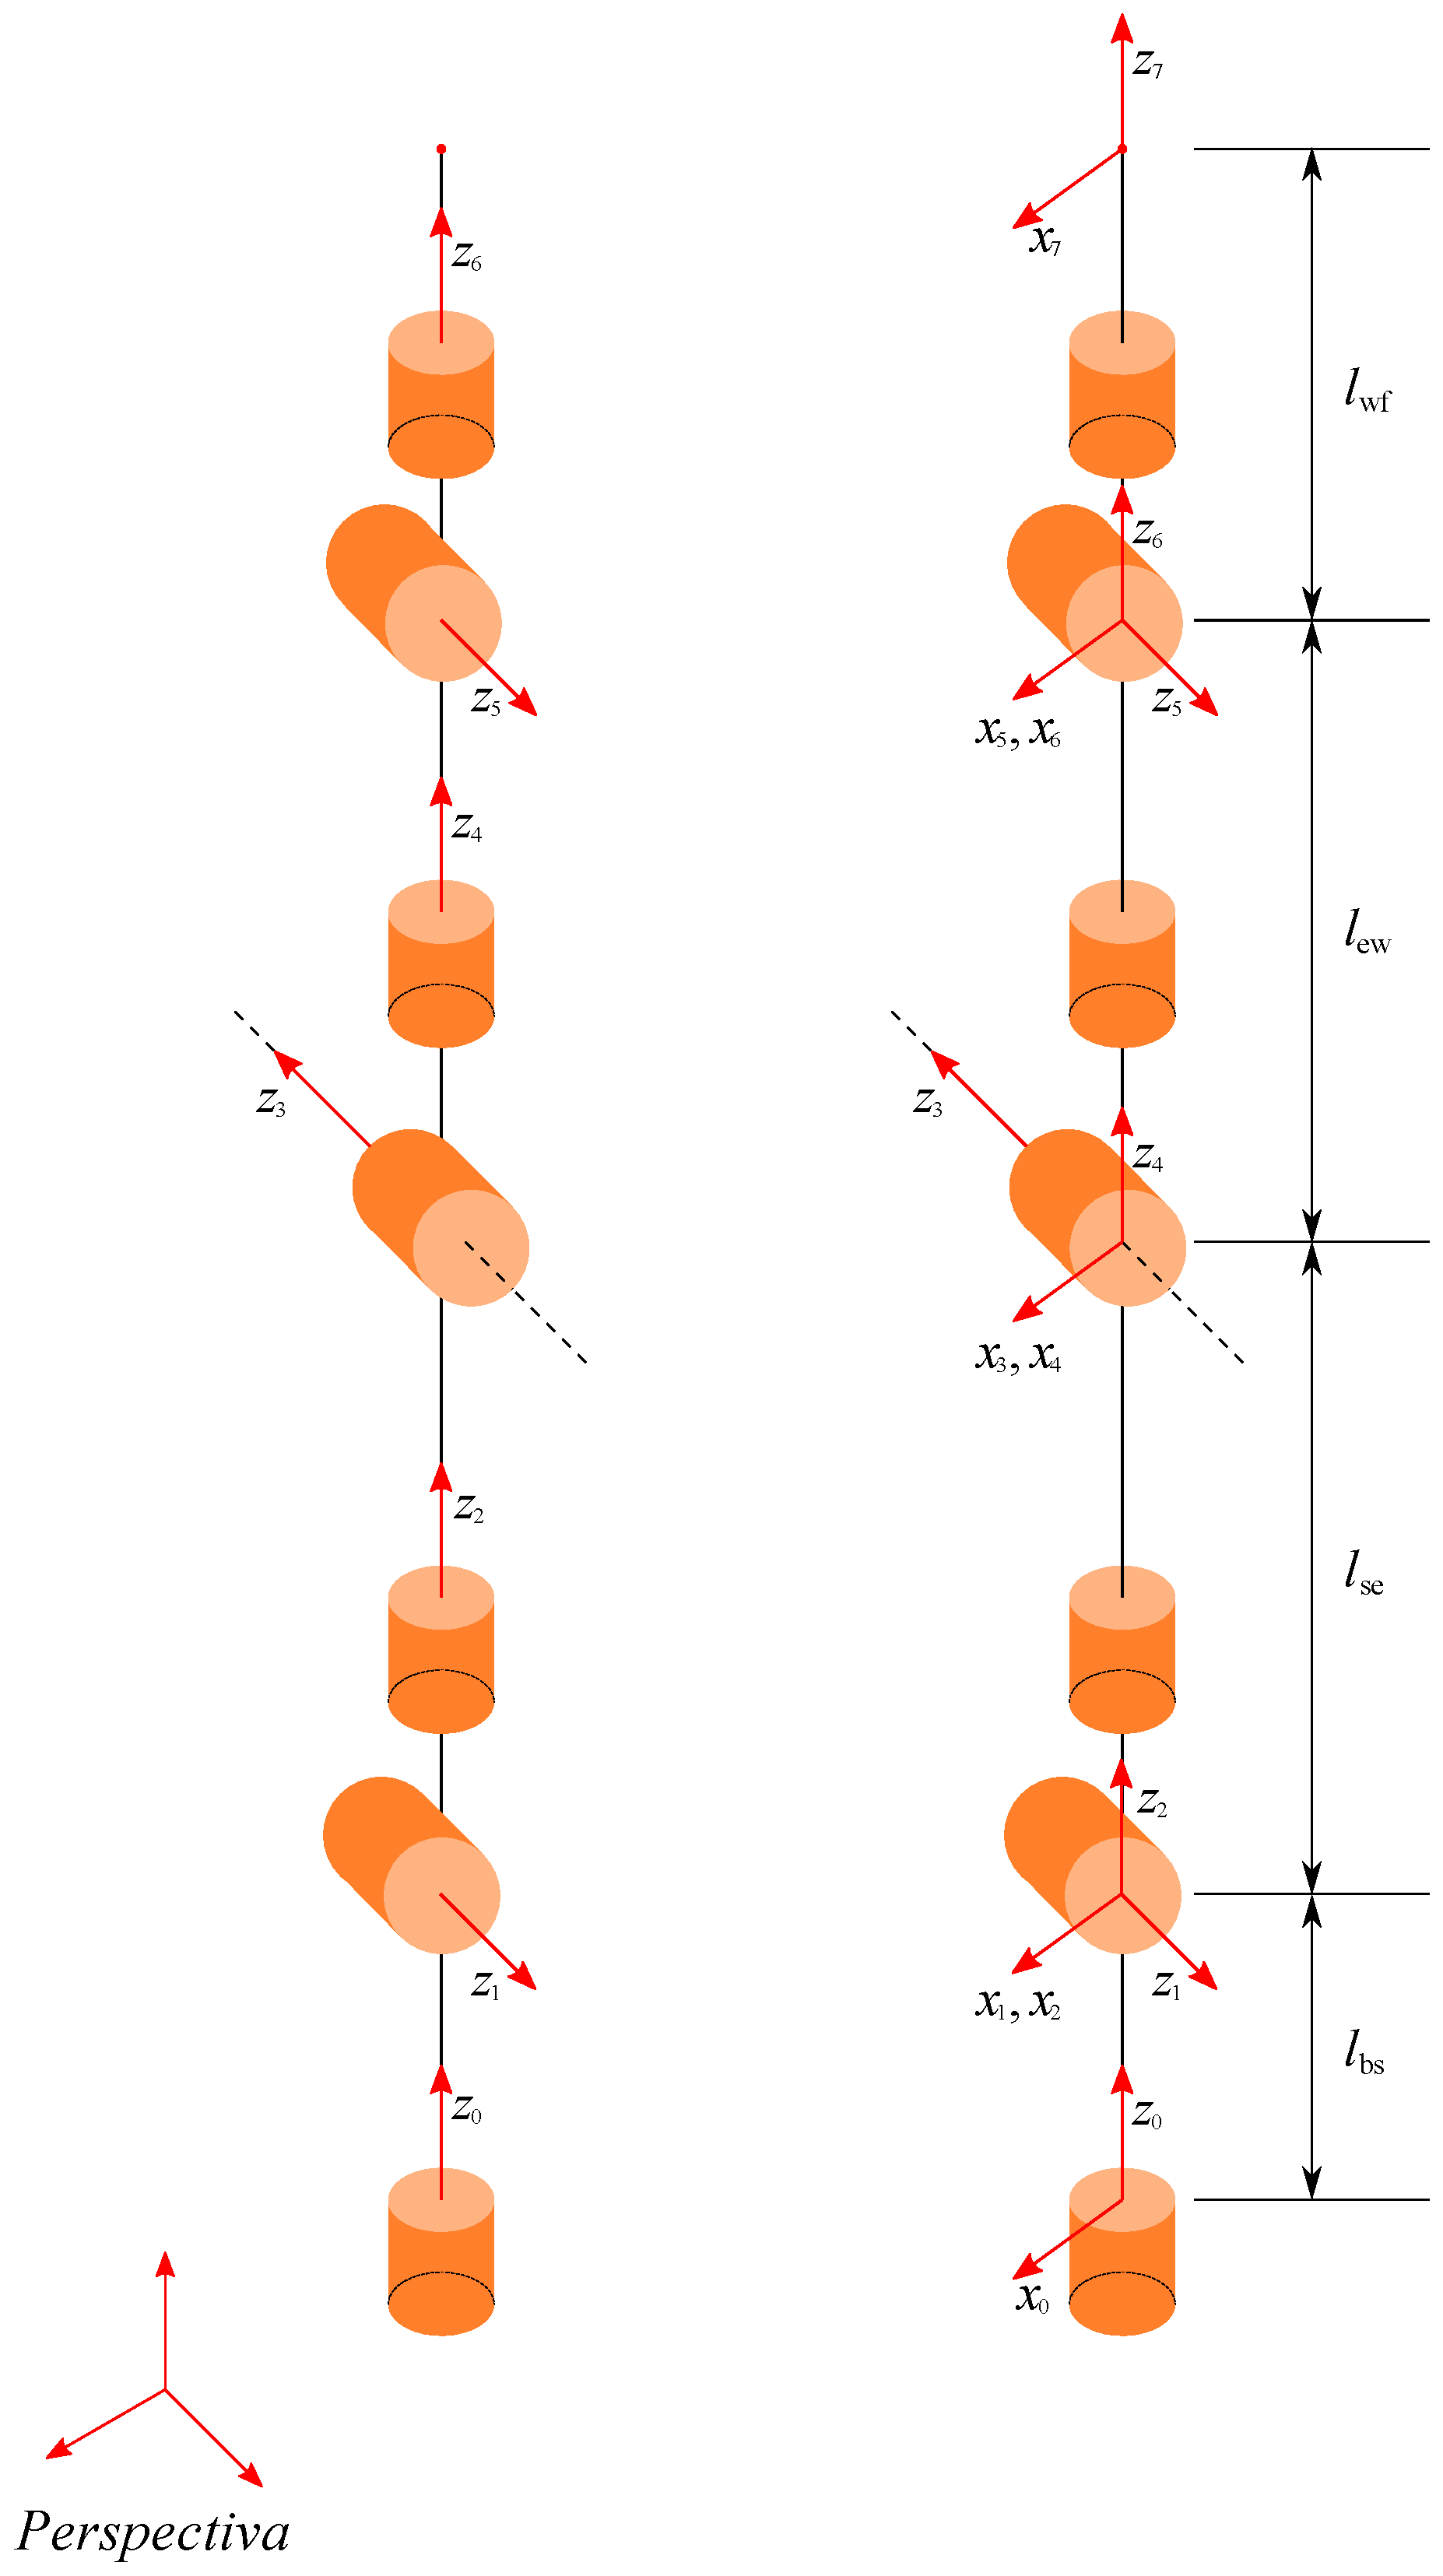
\includegraphics[width=0.7\textwidth]{Fig/x.eps}
\end{minipage}
\end{frame}

\begin{frame}
\frametitle{Tabela de Denavit-Hartenberg}
\begin{minipage}{0.58\textwidth}
%Se $a_i$ é a distância entre $z_{i-1}$ e $z_i$ medido ao longo de $x_i$; $\alpha_i$ o ângulo entre $z_{i-1}$ e $z_i$ mensurado no plano normal a $x_i$;  $d_i$ a distância perpendicular entre a origem $o_{i-1}$ e a interseção de $x_i$ com $z_{i-1}$, medido ao longo de $z_0$; $\theta_i$ o ângulo  entre $x_0$ e $x_1$ mensurado no plano normal a $z_0$.

Os parâmetros dos \textit{links} do KUKA LBR iiwa podem ser retirados da sua interpretação física da atribuição de frames.
\begin{table}[h]
    \centering
    \caption{Parâmetros DH do KUKA LBR iiwa}
    \label{tab:DH}
    \begin{tabular}{crrrr}
    \toprule
        $i$ & $a_i$ & $\alpha_i$ & $d_i$ & $\theta_i$ \\
    \midrule
        1 & 0 & $-\pi/2$ & $\ell_\mathrm{bs}$ & $\theta_1^*$ \\
        2 & 0 &  $\pi/2$ &                  0 & $\theta_2^*$ \\
        3 & 0 &  $\pi/2$ & $\ell_\mathrm{se}$ & $\theta_3^*$ \\
        4 & 0 & $-\pi/2$ &                  0 & $\theta_4^*$ \\
        5 & 0 & $-\pi/2$ & $\ell_\mathrm{ew}$ & $\theta_5^*$ \\
        6 & 0 &  $\pi/2$ &                  0 & $\theta_6^*$ \\
        7 & 0 &        0 & $\ell_\mathrm{wf}$ & $\theta_7^*$ \\
    \bottomrule
    \end{tabular}
    
O $^*$ indica que é variável.
\end{table}
\end{minipage}
\hfill
\begin{minipage}{0.38\textwidth}
    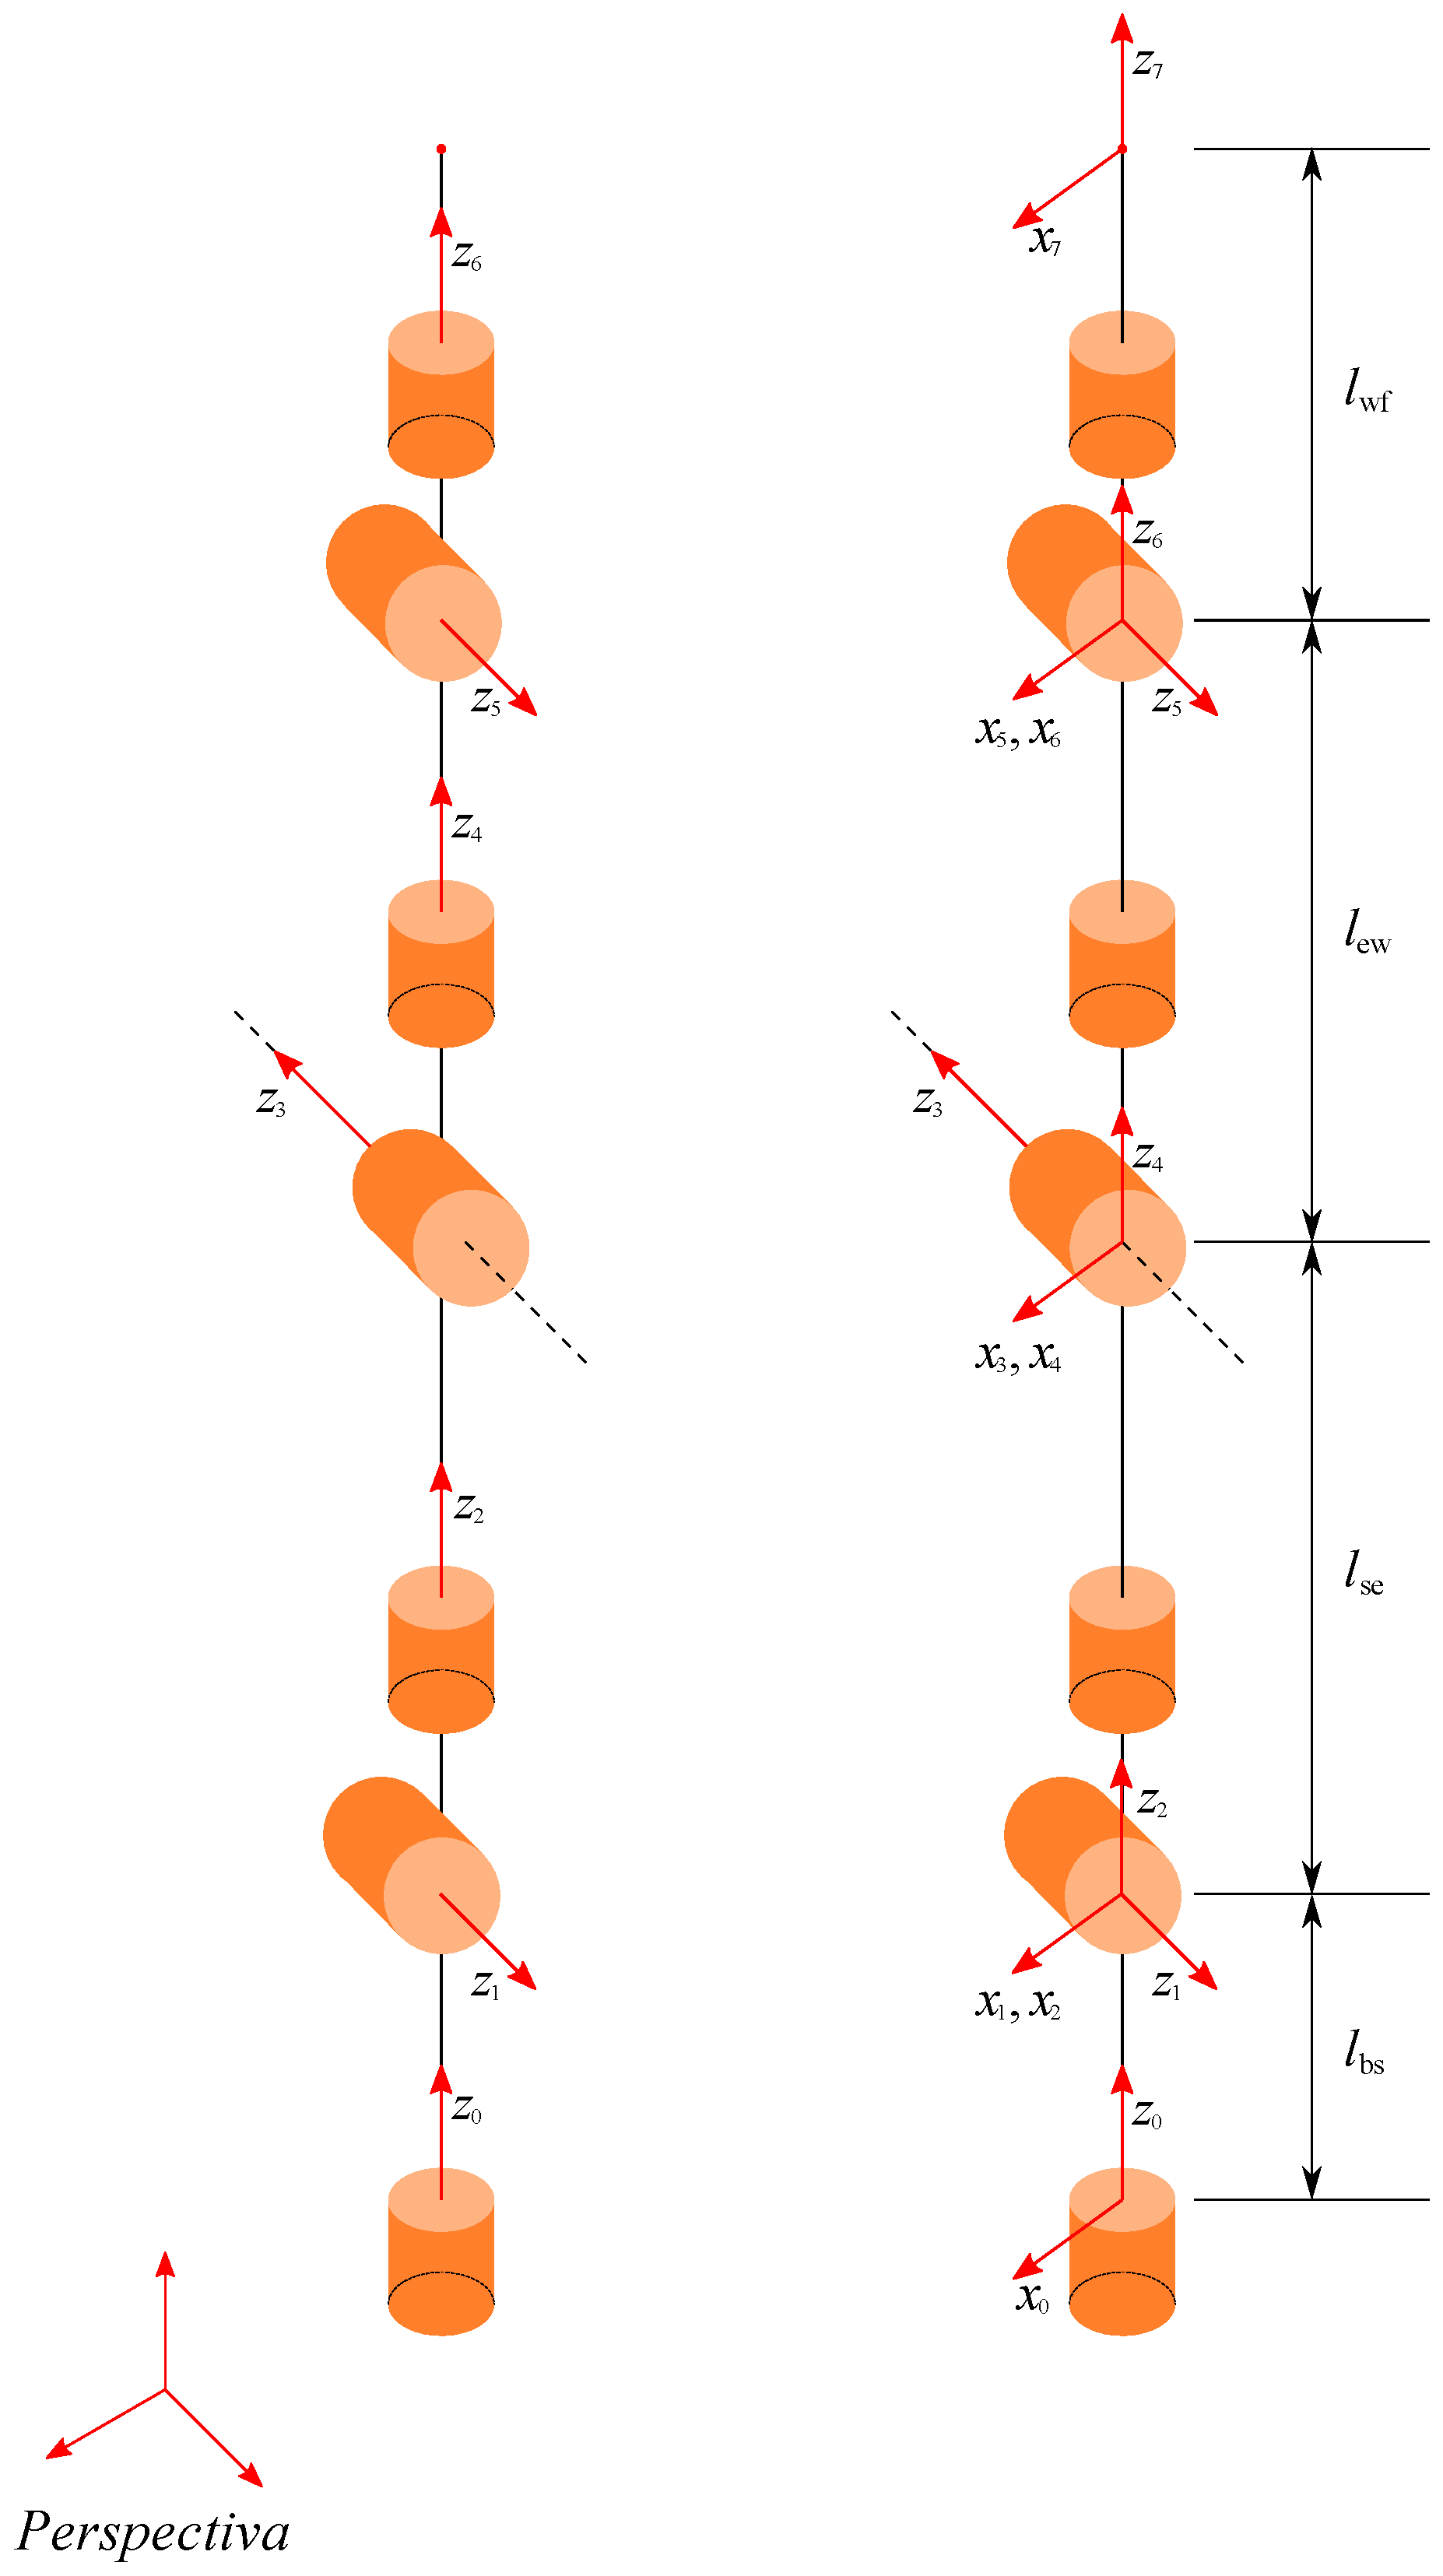
\includegraphics[width=0.7\textwidth]{Fig/x.eps}
\end{minipage}
\end{frame}

%---------------------------------------------------------


%---------------------------------------------------------
\begin{frame}{Matriz de Transformação Homogênea}
Usando os parâmetros obtidos na tabela, em cada linha é obtida a matriz de transformação homogênea $A_i$ do \textit{link} $i$ para o \textit{link} $i-1$, fazendo
\begin{align*}
  \setlength{\dashlinegap}{2pt}
    A_i
    &= \Rot_{z,\,\theta_i} \Trans_{z,\,d_i} \Trans_{x,\,a_i} \Rot_{x,\,\alpha_i} \\
    &=
    \left[ 
    \begin{array}{rrr;{2pt/2pt}c}
        c_{\theta_i} & -s_{\theta_i}c_{\alpha_i} & s_{\theta_i} s_{\alpha_i} & a_i c_{\theta_i} \\
        s_{\theta_i} & c_{\theta_i} c_{\alpha} & -c_{\theta_i} s_{\alpha} & a_i s_{\theta_i} \\
        0 & s_{\alpha_i} & c_{\alpha_i} & d_i \\
        \hdashline[2pt/2pt]
        0 & 0 & 0 & 1
    \end{array}
    \right]
\end{align*}
A matriz de transformação $T$ de $n$ para 0 é então determinada por
\begin{equation*}
    T_n^0 = \prod_{i=0}^n A_i
\end{equation*}
\end{frame}
\begin{frame}{Matriz de Transformação Homogênea}
\begin{minipage}{0.48\textwidth}
Para o \textit{link} 1, segue $a_1 = 0$, $\alpha_1 = -\pi/2$, $d_1=\ell_\mathrm{bs}$ e $\theta_1$ sendo a variável, então
\begin{align*}
    A_1 
    &=
    \left[ 
    \begin{array}{rrr;{2pt/2pt}c}
        c_{\theta_1} & 0 & -s_{\theta_1} & 0 \\
        s_{\theta_1} & 0 &  c_{\theta_1} & 0 \\
        0 & -1 & 0 & \ell_\mathrm{bs} \\
        \hdashline[2pt/2pt]
        0 & 0 & 0 & 1
    \end{array}
    \right]
\end{align*}
Para o \textit{link} 2, segue $a_2 = 0$, $\alpha_2 = \pi/2$, $d_2=0$ e $\theta_2$ sendo a variável, então
\begin{align*}
    A_2 &=
    \left[ 
    \begin{array}{rrr;{2pt/2pt}c}
        c_{\theta_2} & 0 &  s_{\theta_2} & 0 \\
        s_{\theta_2} & 0 & -c_{\theta_2} & 0 \\
        0 & 1 & 0 &  0 \\
        \hdashline[2pt/2pt]
        0 & 0 & 0 & 1
    \end{array}
    \right]
\end{align*}
\end{minipage}
\hfill
\begin{minipage}{0.48\textwidth}
Para o \textit{link} 3, segue $a_3 = 0$, $\alpha_3 = \pi/2$, $d_3=\ell_\mathrm{se}$ e $\theta_3$ sendo a variável, então
\begin{align*}
    A_3 &=
    \left[ 
    \begin{array}{rrr;{2pt/2pt}c}
        c_{\theta_3} & 0 &  s_{\theta_3} & 0 \\
        s_{\theta_3} & 0 & -c_{\theta_3} & 0 \\
        0 & 1 & 0 &  \ell_\mathrm{se} \\
        \hdashline[2pt/2pt]
        0 & 0 & 0 & 1
    \end{array}
    \right]
\end{align*}
Para o \textit{link} 4, segue $a_4 = 0$, $\alpha_4 = -\pi/2$, $d_4=0$ e $\theta_4$ sendo a variável, então
\begin{align*}
    A_4 
    &=
    \left[ 
    \begin{array}{rrr;{2pt/2pt}c}
        c_{\theta_4} & 0 & -s_{\theta_4} & 0 \\
        s_{\theta_4} & 0 &  c_{\theta_4} & 0 \\
        0 & -1 & 0 & 0 \\
        \hdashline[2pt/2pt]
        0 & 0 & 0 & 1
    \end{array}
    \right]
\end{align*}
\end{minipage}
\end{frame}

\begin{frame}{Matriz de Transformação Homogênea}
\begin{minipage}{0.48\textwidth}
Para o \textit{link} 5, segue $a_5 = 0$, $\alpha_5 = -\pi/2$, $d_5=\ell_\mathrm{ew}$ e $\theta_5$ sendo a variável, então
\begin{align*}
    A_5 &=
    \left[ 
    \begin{array}{rrr;{2pt/2pt}c}
        c_{\theta_5} & 0 & -s_{\theta_5} & 0 \\
        s_{\theta_5} & 0 &  c_{\theta_5} & 0 \\
        0 & -1 & 0 &  \ell_\mathrm{ew} \\
        \hdashline[2pt/2pt]
        0 & 0 & 0 & 1
    \end{array}
    \right]
\end{align*}
Para o \textit{link} 6, segue $a_6 = 0$, $\alpha_6 = \pi/2$, $d_6=0$ e $\theta_6$ sendo a variável, então
\begin{align*}
    A_6 &=
    \left[ 
    \begin{array}{rrr;{2pt/2pt}c}
        c_{\theta_6} & 0 &  s_{\theta_6} & 0 \\
        s_{\theta_6} & 0 & -c_{\theta_6} & 0 \\
        0 & 1 & 0 &  0 \\
        \hdashline[2pt/2pt]
        0 & 0 & 0 & 1
    \end{array}
    \right]
\end{align*}
\end{minipage}
\hfill
\begin{minipage}{0.48\textwidth}
Para o \textit{link} 7, $a_7 = 0$, $\alpha_7 = 0$, $d_7=\ell_\mathrm{wf}$ e sendo $\theta_7$ a variável, segue
    \begin{align*}
        A_7 =
        \left[ 
    \begin{array}{rrr;{2pt/2pt}c}
        c_{\theta_7} & -s_{\theta_7} & 0 & 0 \\
        s_{\theta_7} &  c_{\theta_7} & 0 & 0 \\
        0 & 0 & 1 & \ell_\mathrm{wf} \\
        \hdashline[2pt/2pt]
        0 & 0 & 0 & 1
    \end{array}
    \right]
    \end{align*}
\end{minipage}
\end{frame}
\begin{frame}{Matriz de Transformação Homogênea}
    Por fim, a matriz de transformação homogênea do frame 7 para o frame 0 é encontrada fazendo
    \begin{equation}
        T_7^0 = A_1 A_2 A_3 A_4 A_5 A_6 A_7
    \end{equation}
uma multiplicação de 7 matrizes $4\times4$ de variáveis reais.
\end{frame}

%% Caso se queira retirar as matrizes, comente a linha de código abaixo
%\subsection{Matriz de Transformação}
\begin{frame}{Matriz de Transformação}
A multiplicação das matrizes $n$ matrizes de transformação homogênea resulta em
\begin{equation}
    T_{n}^0 =
    \left[
    \begin{array}{ccc;{2pt/2pt}c}
        r_{11} & r_{12} & r_{13} & d_x \\
        r_{21} & r_{22} & r_{33} & d_y \\
        r_{31} & r_{22} & r_{33} & d_z \\        \hdashline[2pt/2pt]
             0 &      0 &      0 &    1
    \end{array}
    \right]
\end{equation}
Para a qual os termos serão expostos a seguir.
\end{frame}
\begingroup
\footnotesize
\begin{frame}{Rotação}
\begin{multline*}
    r_{11} =
    \Bigg[\Big[ \left(\left(- s_1 s_3 + c_1 c_2 c_3\right) c_4 + s_2 s_4 c_1\right) c_5 + \left(- s_1 c_3 - s_3 c_1 c_2\right) s_5 \Big] c_6 + \\
    %%
    %%
    \left(\left(- s_1 s_3 + c_1 c_2 c_3\right) s_4 - s_2 c_1 c_4\right) s_6\Bigg] c_7 + \Bigg[- \Big[\left(- s_1 s_3 + c_1 c_2 c_3\right) c_4 + \\
    %%
    %%
    s_2 s_4 c_1\Big] s_5 + \left(- s_1 c_3 - s_3 c_1 c_2\right) c_5\Bigg] s_7
\end{multline*}
\begin{multline*}
    r_{12} = - \Bigg[\Big[\left(\left(- s_1 s_3 + c_1 c_2 c_3\right) c_4 + s_2 s_4 c_1\right) c_5 + \left(- s_1 c_3 - s_3 c_1 c_2\right) s_5\Big] c_6 \\
    %%
    %%
    + \left(\left(- s_1 s_3 + c_1 c_2 c_3\right) s_4 - s_2 c_1 c_4\right) s_6\Bigg] s_7 + \Bigg[- \Big[\left(- s_1 s_3 + c_1 c_2 c_3\right) c_4 \\
    %%
    %%
    + s_2 s_4 c_1\Big] s_5 + \left(- s_1 c_3 - s_3 c_1 c_2\right) c_5\Bigg] c_7
\end{multline*}
\end{frame}

\begin{frame}{Rotação}
\begin{multline*}
r_{13} = 
\Big[\left(\left(- s_1 s_3 + c_1 c_2 c_3\right) c_4 + s_2 s_4 c_1\right) c_5 + \left(- s_1 c_3 - s_3 c_1 c_2\right) s_5\Big] s_6\\
%%
%%
- \left(\left(- s_1 s_3 + c_1 c_2 c_3\right) s_4 - s_2 c_1 c_4\right) c_6
\end{multline*}
\begin{multline*}
    r_{21} = \Bigg[\Big[\left(\left(s_1 c_2 c_3 + s_3 c_1\right) c_4 + s_1 s_2 s_4\right) c_5 + \left(- s_1 s_3 c_2 + c_1 c_3\right) s_5\Big] c_6 \\
    %%
    %%
    + \left(\left(s_1 c_2 c_3 + s_3 c_1\right) s_4 - s_1 s_2 c_4\right) s_6\Bigg] c_7 + \Bigg[- \Big[\left(s_1 c_2 c_3 + s_3 c_1\right) c_4 \\
    %%
    %%
    + s_1 s_2 s_4\Big] s_5 + \left(- s_1 s_3 c_2 + c_1 c_3\right) c_5\Bigg] s_7
\end{multline*}
\end{frame}
\begin{frame}{Rotação}
    \begin{multline*}
        r_{22} = - \Bigg[\Big[\left(\left(s_1 c_2 c_3 + s_3 c_1\right) c_4 + s_1 s_2 s_4\right) c_5 + \left(- s_1 s_3 c_2 + c_1 c_3\right) s_5\Big] c_6 \\
        %%
        %%
        + \left(\left(s_1 c_2 c_3 + s_3 c_1\right) s_4 - s_1 s_2 c_4\right) s_6\Bigg] s_7 + \Bigg[- \Big[\left(s_1 c_2 c_3 + s_3 c_1\right) c_4 \\
        %%
        %%
        + s_1 s_2 s_4\Big] s_5 + \left(- s_1 s_3 c_2 + c_1 c_3\right) c_5 \Bigg] c_7
    \end{multline*}
    \begin{multline*}
        r_{23} = 
        \Bigg[\Big[\left(s_1 c_2 c_3 + s_3 c_1\right) c_4 + s_1 s_2 s_4\Big] c_5 + \left(- s_1 s_3 c_2 + c_1 c_3\right) s_5\Bigg] s_6 \\
        %%
        %%
        - \Big[\left(s_1 c_2 c_3 + s_3 c_1\right) s_4 - s_1 s_2 c_4\Big] c_6
    \end{multline*}
\end{frame}
\begin{frame}{Rotação}
\begin{multline*}
r_{31} =
    \Big[\left(\left(- s_2 c_3 c_4 + s_4 c_2\right) c_5 + s_2 s_3 s_5\right) c_6 + \left(- s_2 s_4 c_3 - c_2 c_4\right) s_6\Big] c_7 \\
    + \Big[- \left(- s_2 c_3 c_4 + s_4 c_2\right) s_5 + s_2 s_3 c_5\Big] s_7
\end{multline*}
\begin{multline*}
r_{32} =
    - \Big[\left(\left(- s_2 c_3 c_4 + s_4 c_2\right) c_5 + s_2 s_3 s_5\right) c_6 + \left(- s_2 s_4 c_3 - c_2 c_4\right) s_6\Big] s_7 \\
    + \Big[- \left(- s_2 c_3 c_4 + s_4 c_2\right) s_5 + s_2 s_3 c_5\Big] c_7
\end{multline*}
\begin{flalign*}
r_{33} =
    \Big[ \left(- s_2 c_3 c_4 + s_4 c_2\right) c_5 + s_2 s_3 s_5\Big] s_6 - \left(- s_2 s_4 c_3 - c_2 c_4\right) c_6
\end{flalign*}
\end{frame}


\begin{frame}{Translação}
    \begin{multline*}
    d_{x} = 90 \Big[\left(\left(- s_1 s_3 + c_1 c_2 c_3\right) c_4 + s_2 s_4 c_1\right) c_5 + \left(- s_1 c_3 - s_3 c_1 c_2\right) s_5\Big] s_6 \\
    %%
    %%
    - 90 \Big[\left(- s_1 s_3 + c_1 c_2 c_3\right) s_4 - s_2 c_1 c_4\Big] c_6 - 400 \left(- s_1 s_3 + c_1 c_2 c_3\right) s_4 \\
    %%
    %%
    +400 s_2 c_1 c_4 + 420 s_2 c_1
\end{multline*}
\begin{multline*}
    d_y =
    90 \Big[\left(\left(s_1 c_2 c_3 + s_3 c_1\right) c_4 + s_1 s_2 s_4\right) c_5 + \left(- s_1 s_3 c_2 + c_1 c_3\right) s_5 \Big] s_6 \\
    %%
    %%
    - 90 \Big[\left(s_1 c_2 c_3 + s_3 c_1\right) s_4 - s_1 s_2 c_4\Big] c_6 - 400 \left(s_1 c_2 c_3 + s_3 c_1\right) s_4 \\
    + 400 s_1 s_2 c_4 + 420 s_1 s_2
\end{multline*}
\begin{multline*}
    d_z = 90 \Big[\left(- s_2 c_3 c_4 + s_4 c_2\right) c_5 + s_2 s_3 s_5\Big] s_6 - 90 \left(- s_2 s_4 c_3 - c_2 c_4\right) c_6 \\
    %%
    %%
    + 400 s_2 s_4 c_3 + 400 c_2 c_4 + 420 c_2 + 360
\end{multline*}
\end{frame}
\endgroup

%---------------------------------------------------------

\section{Validação}

%---------------------------------------------------------
%Highlighting text
\begin{frame}
\frametitle{Implementação: \textit{Set Up}}
\begin{mintedbox}{python}
import sympy as sp    # Pacote para manipulaçoes simbolicas
from sympy import pi, sin, cos
from sympy.physics.vector import init_vprinting   # Usada para printar em latex
from sympy.physics.mechanics import dynamicsymbols

init_vprinting(use_latex='mathjax', pretty_print=False)   # Configurando o vprinting

theta1, theta2, theta3, theta4 = dynamicsymbols('theta1 theta2 theta3 theta4')
theta5, theta6, theta7 = dynamicsymbols('theta5 theta6 theta7')
l1, l2, theta, alpha, a, d = dynamicsymbols('l1 l2 theta alpha a d')
\end{mintedbox}
\end{frame}
%%%%%%%%%%%%%%%%%%%%%%
%%%%%%%%%%%%%%%%%%%%%%
%%%%%%%%%%%%%%%%%%%%%%
%%%%%%%%%%%%%%%%%%%%%%
\begin{frame}
\frametitle{Implementação: Tabela DH}
\begin{mintedbox}{python}
# Valores das distancias (LBR iiwa 14 820)
dbs, dse, dew, dwf = 360, 420, 400, 90

# Matriz DH:        alfi, ai, di, thetai
TDH = sp.Matrix([ [-pi/2, 0, dbs, theta1],
                  [ pi/2, 0,   0, theta2],
                  [ pi/2, 0, dse, theta3],
                  [-pi/2, 0,   0, theta4],
                  [-pi/2, 0, dew, theta5],
                  [ pi/2, 0,   0, theta6],
                  [    0, 0, dwf, theta7]])
\end{mintedbox}
\end{frame}
%%%%%%%%%%%%%%%%%%%%%%
%%%%%%%%%%%%%%%%%%%%%%
%%%%%%%%%%%%%%%%%%%%%%
%%%%%%%%%%%%%%%%%%%%%%
\begin{frame}
\frametitle{Implementação: $A_i$}
\begin{mintedbox}{python}
Rot = sp.Matrix([
    [cos(theta), -sin(theta)*cos(alpha),  sin(theta)*sin(alpha)],
    [sin(theta), cos(theta)*cos(alpha), -cos(theta)*sin(alpha)],
    [ 0, sin(alpha), cos(alpha)]
                ])

Tran = sp.Matrix([a*cos(theta),a*sin(theta),d])
S = sp.Matrix([[0, 0, 0, 1]])

# Matriz Ai geral
A = sp.Matrix.vstack(sp.Matrix.hstack(Rot, Tran), S)
\end{mintedbox}
\end{frame}
%%%%%%%%%%%%%%%%%%%%%%
%%%%%%%%%%%%%%%%%%%%%%
%%%%%%%%%%%%%%%%%%%%%%
%%%%%%%%%%%%%%%%%%%%%%
\begin{frame}
\frametitle{Implementação: MTH $T_7^0$}
\begin{mintedbox}{python}
# Matriz A de cada linha
A1 = A.subs({alpha:TDH[0,0],a:TDH[0,1],d:TDH[0,2],theta:TDH[0,3]})
A2 = A.subs({alpha:TDH[1,0],a:TDH[1,1],d:TDH[1,2],theta:TDH[1,3] })
A3 = A.subs({alpha:TDH[2,0],a:TDH[2,1],d:TDH[2,2],theta:TDH[2,3] })
A4 = A.subs({alpha:TDH[3,0],a:TDH[3,1],d:TDH[3,2],theta:TDH[3,3] })
A5 = A.subs({alpha:TDH[4,0],a:TDH[4,1],d:TDH[4,2],theta:TDH[4,3] })
A6 = A.subs({alpha:TDH[5,0],a:TDH[5,1],d:TDH[5,2],theta:TDH[5,3] })
A7 = A.subs({alpha:TDH[6,0],a:TDH[6,1],d:TDH[6,2],theta:TDH[6,3]})

# Matriz de transf. homogenea de 7 para 0
T = A1*A2*A3*A4*A5*A6*A7
\end{mintedbox}
\end{frame}
%%%%%%%%%%%%%%%%%%%%%%
%%%%%%%%%%%%%%%%%%%%%%
%%%%%%%%%%%%%%%%%%%%%%
%%%%%%%%%%%%%%%%%%%%%%
\begin{frame}
\frametitle{Validação}
\begin{columns}
\column{0.58\textwidth}
\begin{mintedbox}{python}
# Posição Home
Thome = T.subs({ theta1:0, theta2:0, theta3:0, theta4:0, theta5:0, theta6:0, theta7:0 })

# Posição escolhida
q1, q2, q3     = 0, 0, 0
q4, q5, q6, q7 = -pi/2, pi/3, 0, 0

T_ = T.subs({ theta1:q1, theta2:q2, theta3:q3, theta4:q4, theta5:q5, theta6:q6, theta7:q7 })
\end{mintedbox}
\column{0.38\textwidth}
Ao qual retorna
\begin{align*}
    \mathtt{T}_\mathtt{home}
    &=
    \left[
    \begin{array}{ccc;{2pt/2pt}c}
        1 & 0 & 0 & 0 \\
        0 & 1 & 0 & 0 \\
        0 & 0 & 1 & 1270 \\
        \hdashline[2pt/2pt]
        0 & 0 & 0 & 1
    \end{array}
    \right]
\end{align*}
e
\begin{align*}
    \mathtt{T\_} 
    &=
    \left[
    \begin{array}{ccc;{2pt/2pt}c}
        0 & 0 & 1 & 490 \\
        \frac{\sqrt{3}}{2} & \frac{1}{2} & 0 & 0 \\  -\frac{1}{2} & \frac{\sqrt{3}}{2} & 0 & 780 \\
        \hdashline[2pt/2pt]
        0 & 0 & 0 & 1
    \end{array}
    \right]
\end{align*}
\end{columns}
\end{frame}


\begin{frame}{Análise Dimensional: \textit{home}}
\begin{columns}

\column{0.28\textwidth}
\begin{figure}[h]
    \centering
    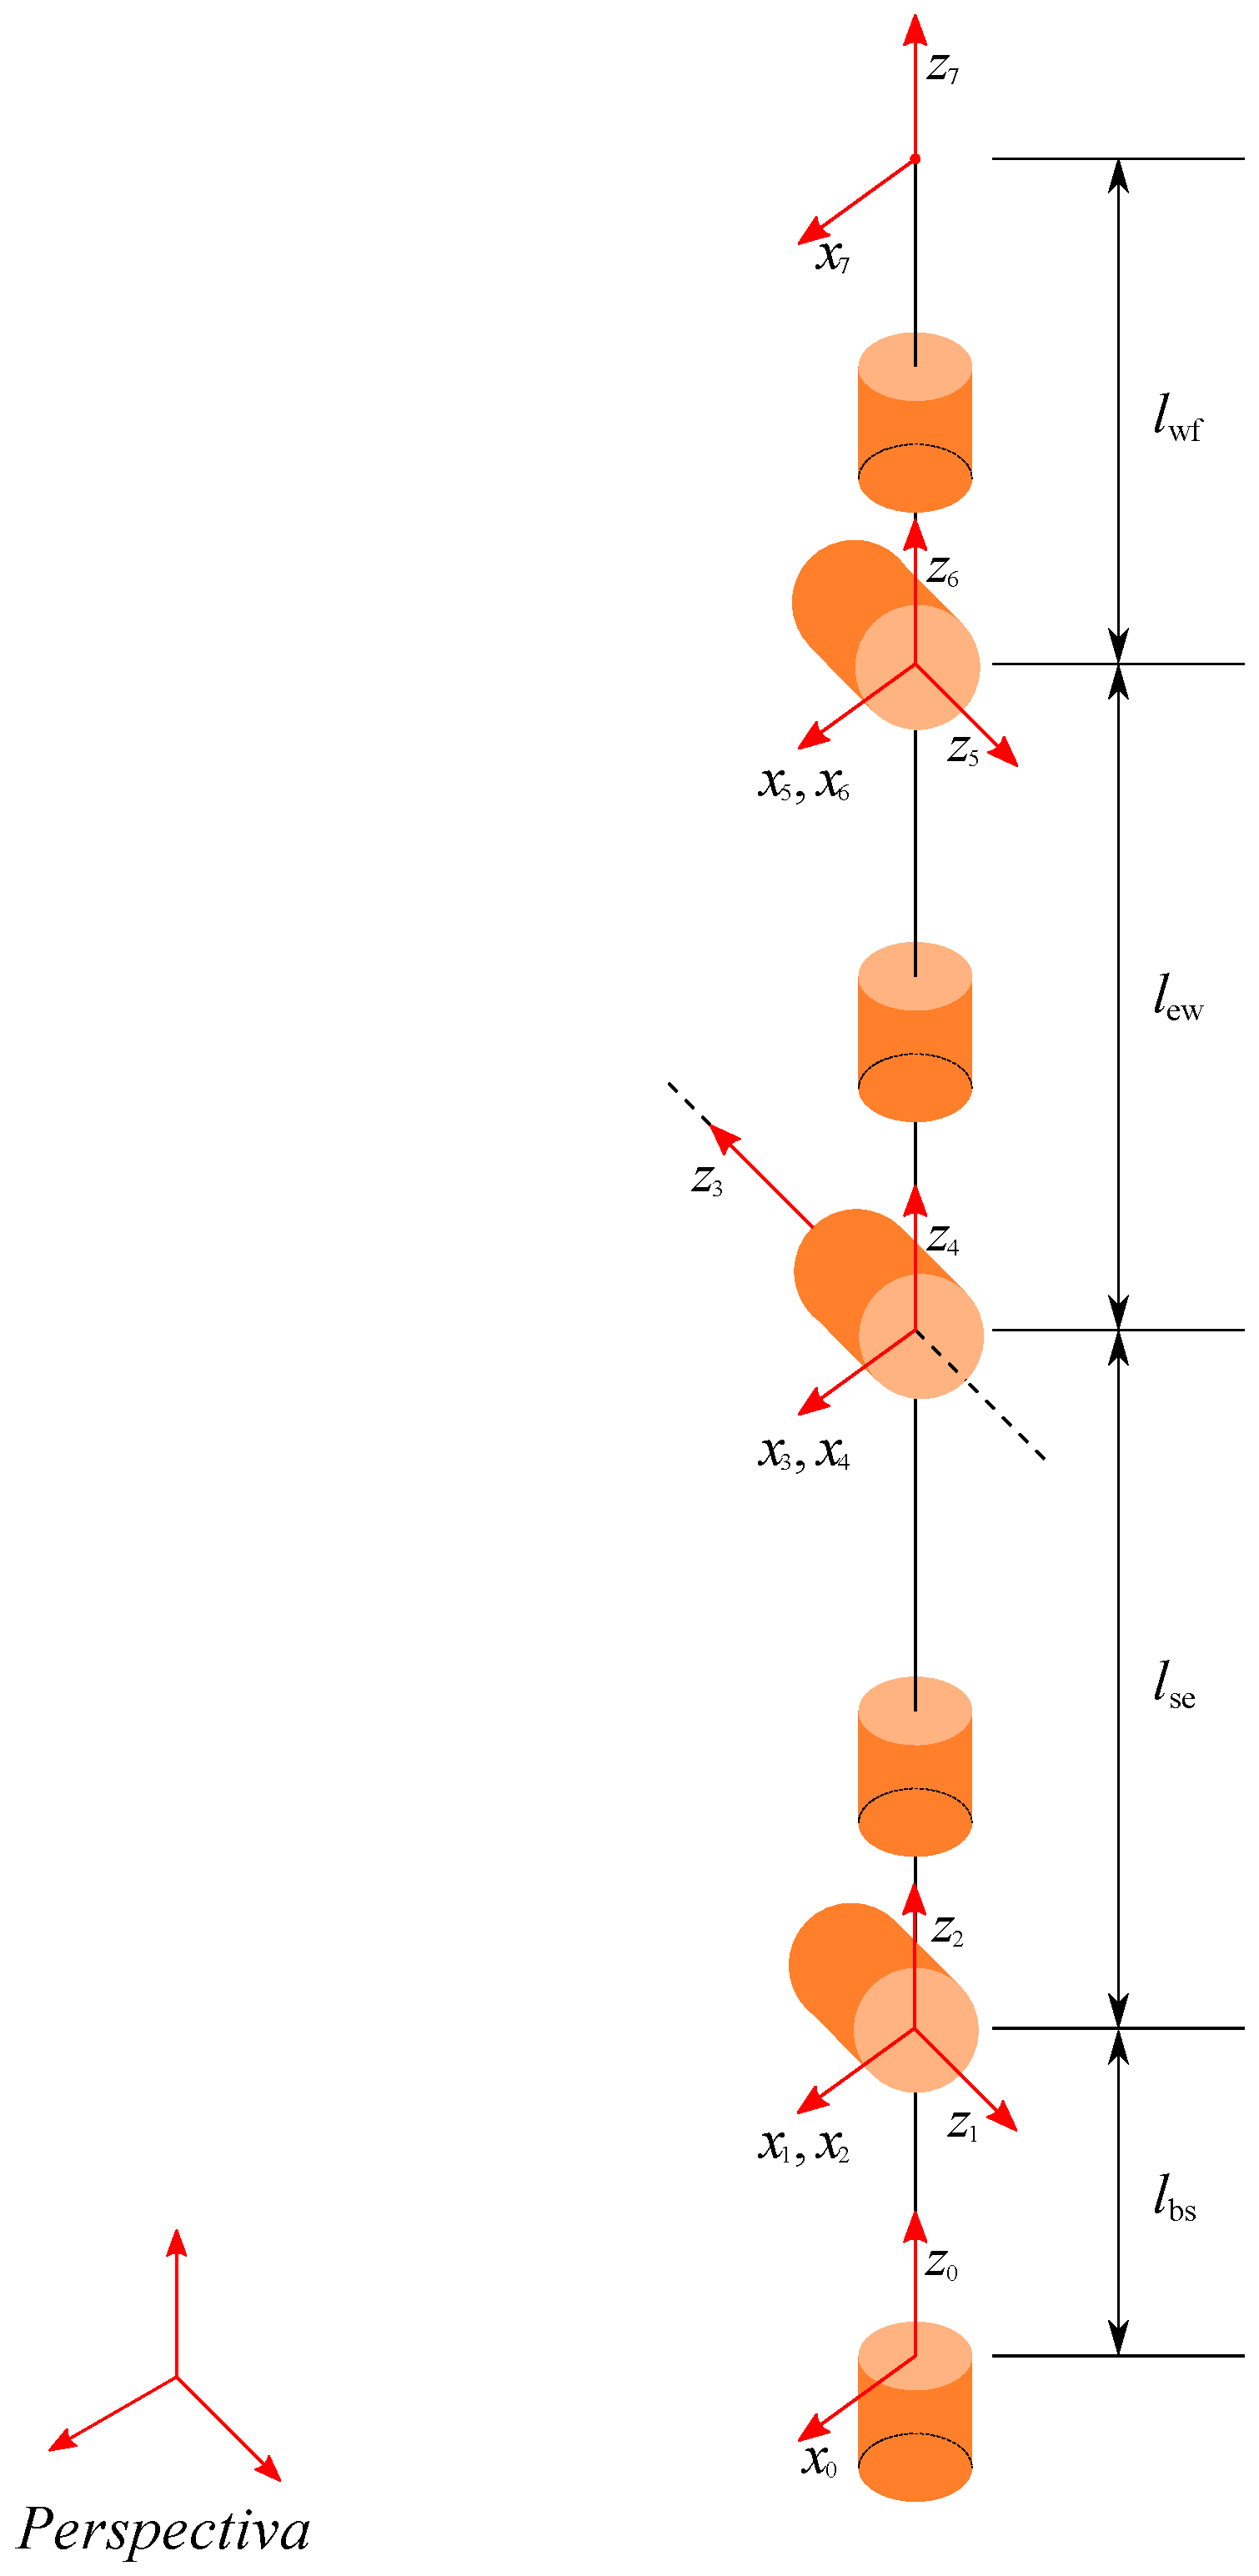
\includegraphics[width=0.75\textwidth,left]{Fig/validacao_home.eps}
\end{figure}

\column{0.68\textwidth}
Para a configuração \textit{home} tem-se
\begin{align*}
    \mathtt{T}_\mathtt{home}
    &=
    \left[
    \begin{array}{ccc;{2pt/2pt}c}
        1 & 0 & 0 & 0 \\
        0 & 1 & 0 & 0 \\
        0 & 0 & 1 & 1270 \\
        \hdashline[2pt/2pt]
        0 & 0 & 0 & 1
    \end{array}
    \right]
\end{align*}

Isto é, uma translação em $z_0$ de 1270 mm e uma rotação de \ang{0}. Como retorna a simulação no RoboDK.

\end{columns}

\end{frame}

\begin{frame}{Análise dimensional da posição escolhida}
\begin{columns}
\column{0.58\textwidth}
Aplicando uma rotação em $\ang{-90}$ na junta 4, o \textit{frame} 4 se torna

\column{0.38\textwidth}
\begin{figure}
    \centering
    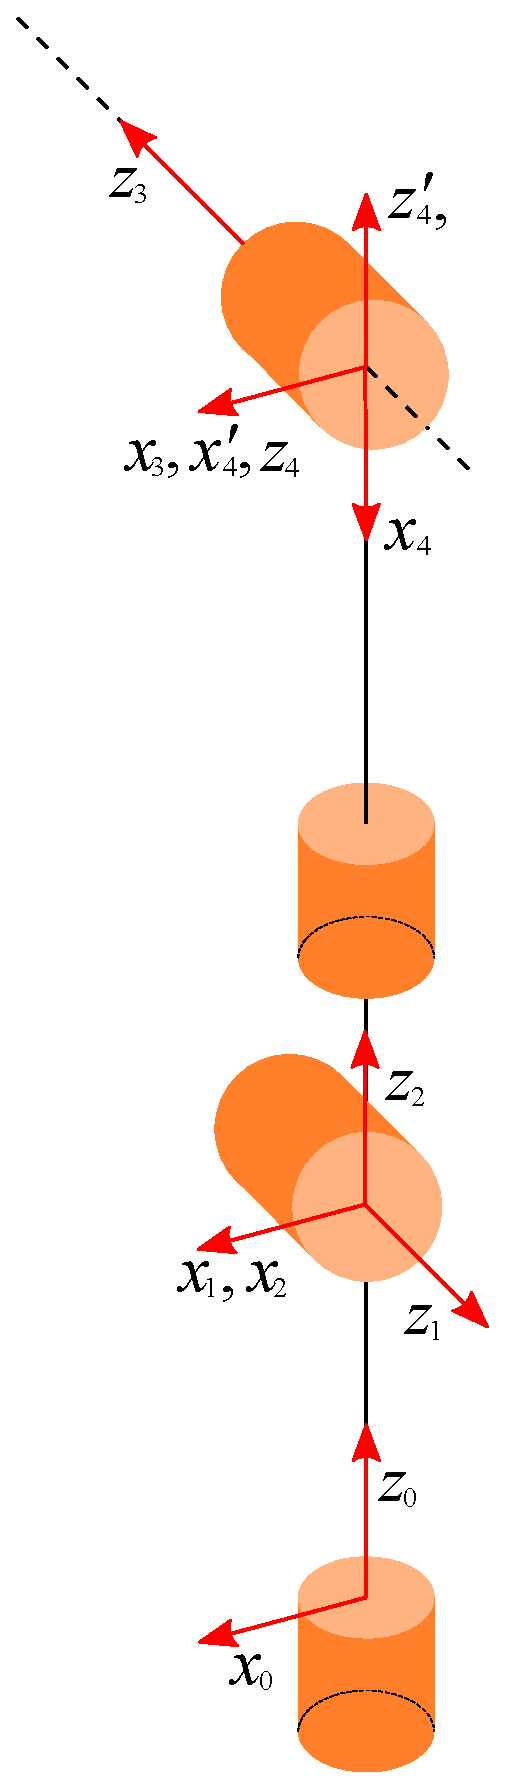
\includegraphics[width=0.3\textwidth,right]{Fig/val_a.eps}
\end{figure}


\end{columns}
\end{frame}

\begin{frame}{Análise dimensional da posição escolhida}
\begin{columns}
\column{0.48\textwidth}
Associando a rotação do frame com o restante do robô temos
\column{0.48\textwidth}
\begin{figure}
    \centering
    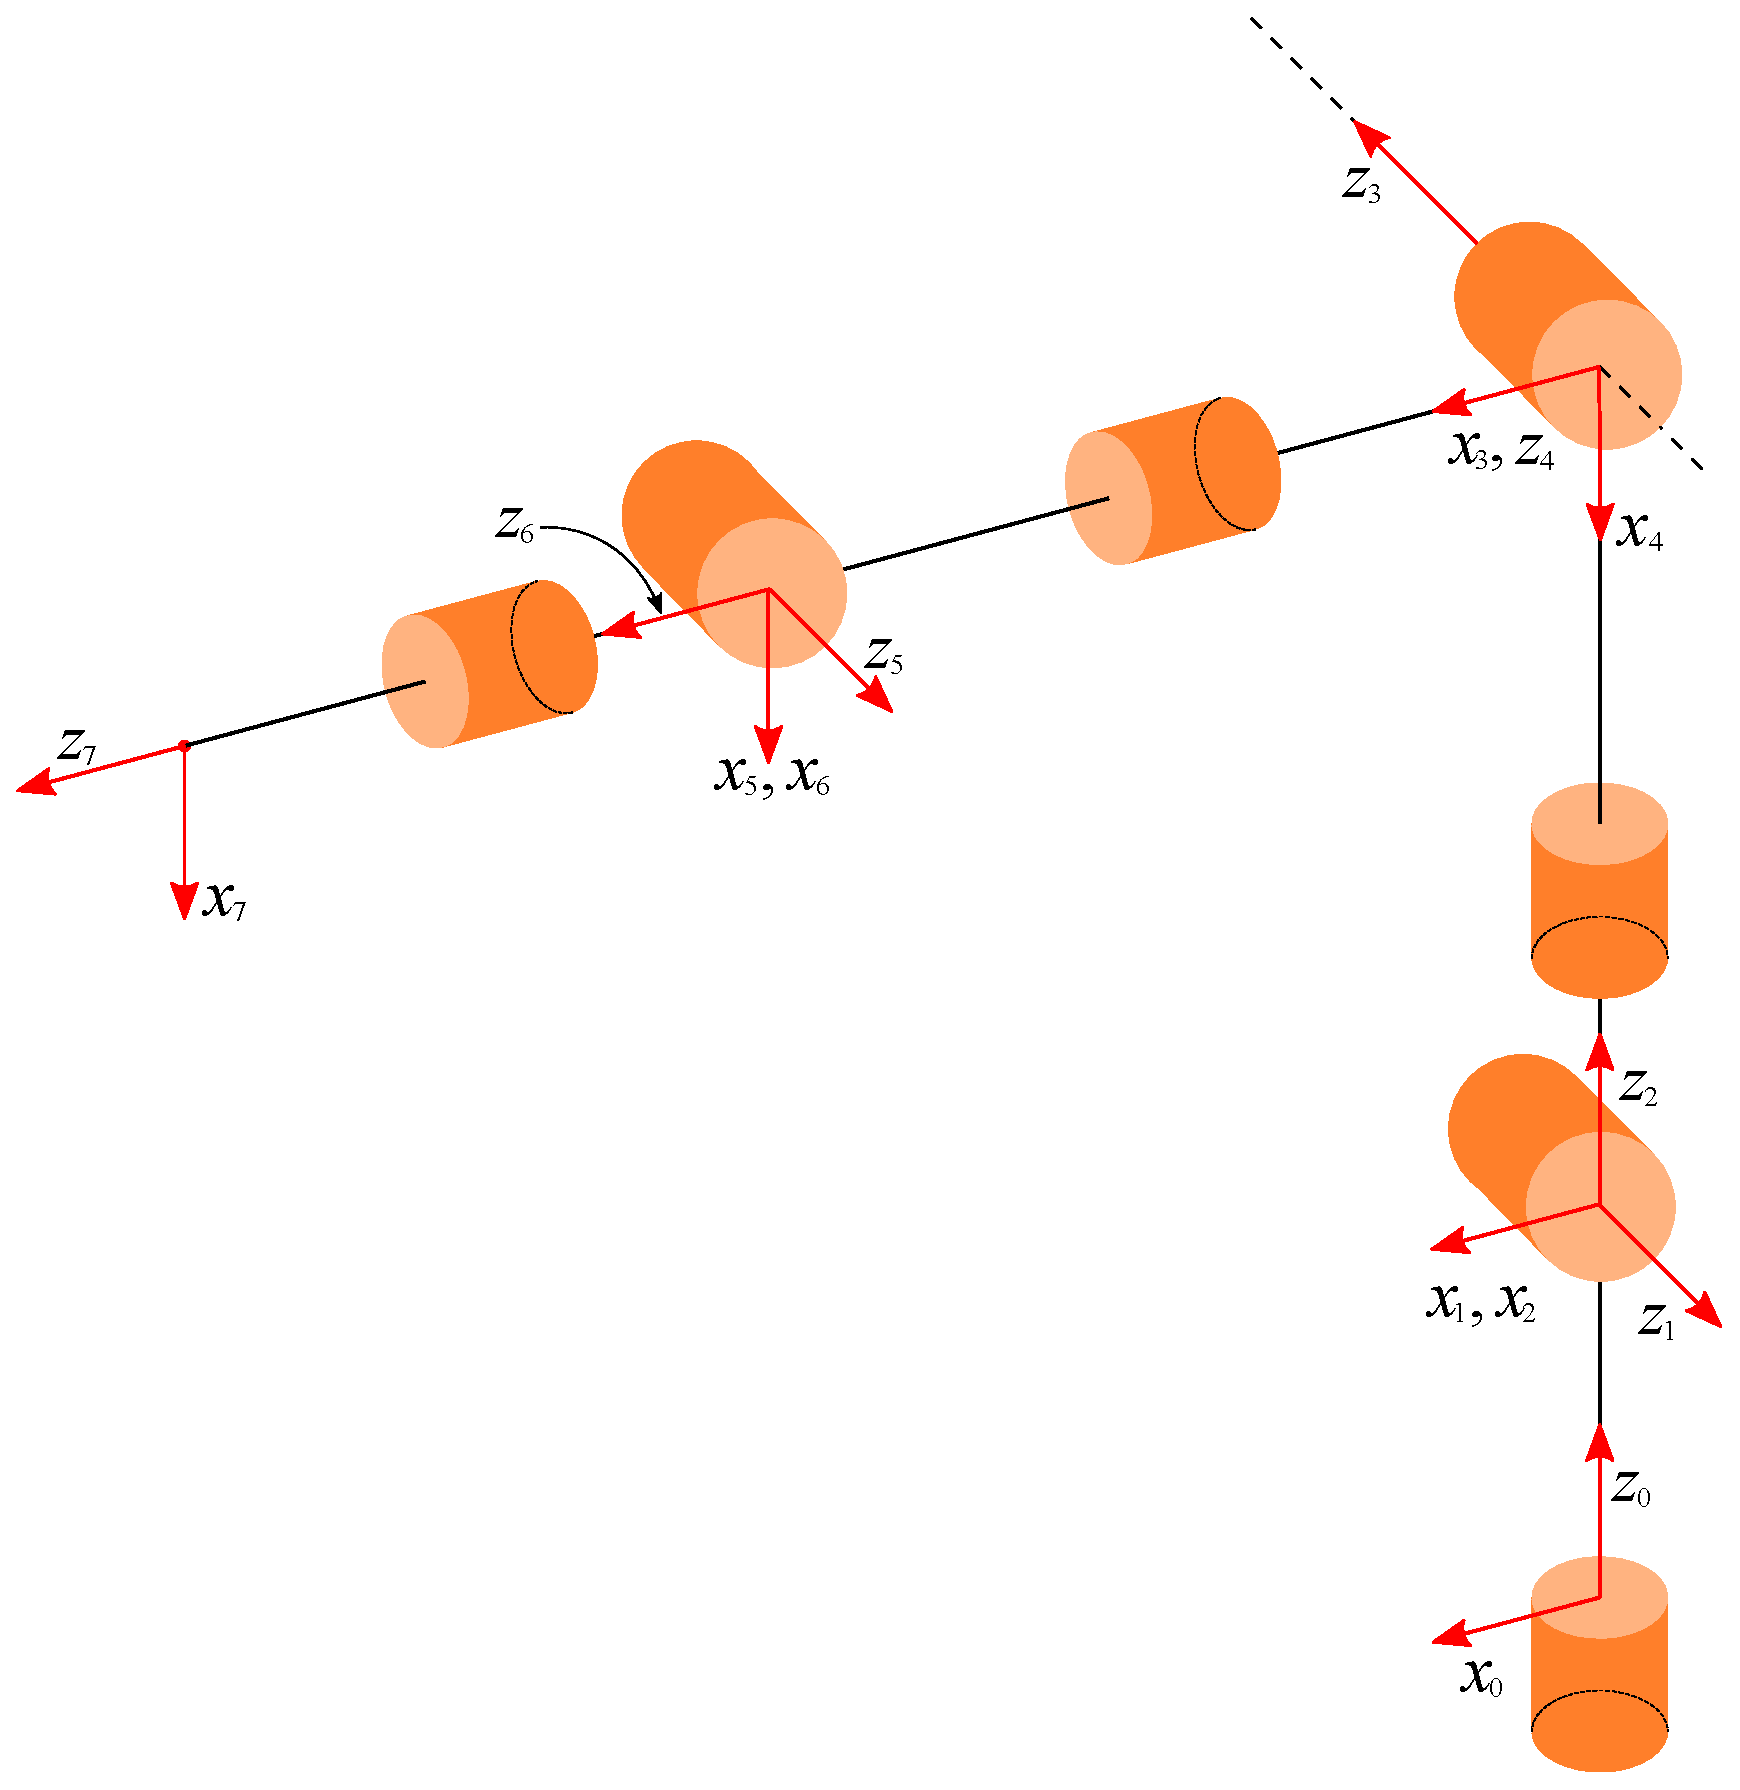
\includegraphics[width=0.85\textwidth,right]{Fig/val_b.eps}
\end{figure}
\end{columns}
\end{frame}

\begin{frame}{Análise dimensional da posição escolhida}
\begin{columns}
\column{0.48\textwidth}
Agora, é feita uma rotação de \ang{60} na junta 5 e o frame 5 se torna

\column{0.48\textwidth}
\begin{figure}
    \centering
    \includegraphics[width=0.65\textwidth,right]{Fig/val_c.eps}
\end{figure}
\end{columns}
\end{frame}

\begin{frame}{Análise dimensional da posição escolhida}
\begin{columns}
\column{0.48\textwidth}
Por fim, a representação final do robô é feita compondo as duas rotações.

\column{0.48\textwidth}
\begin{figure}
    \centering
    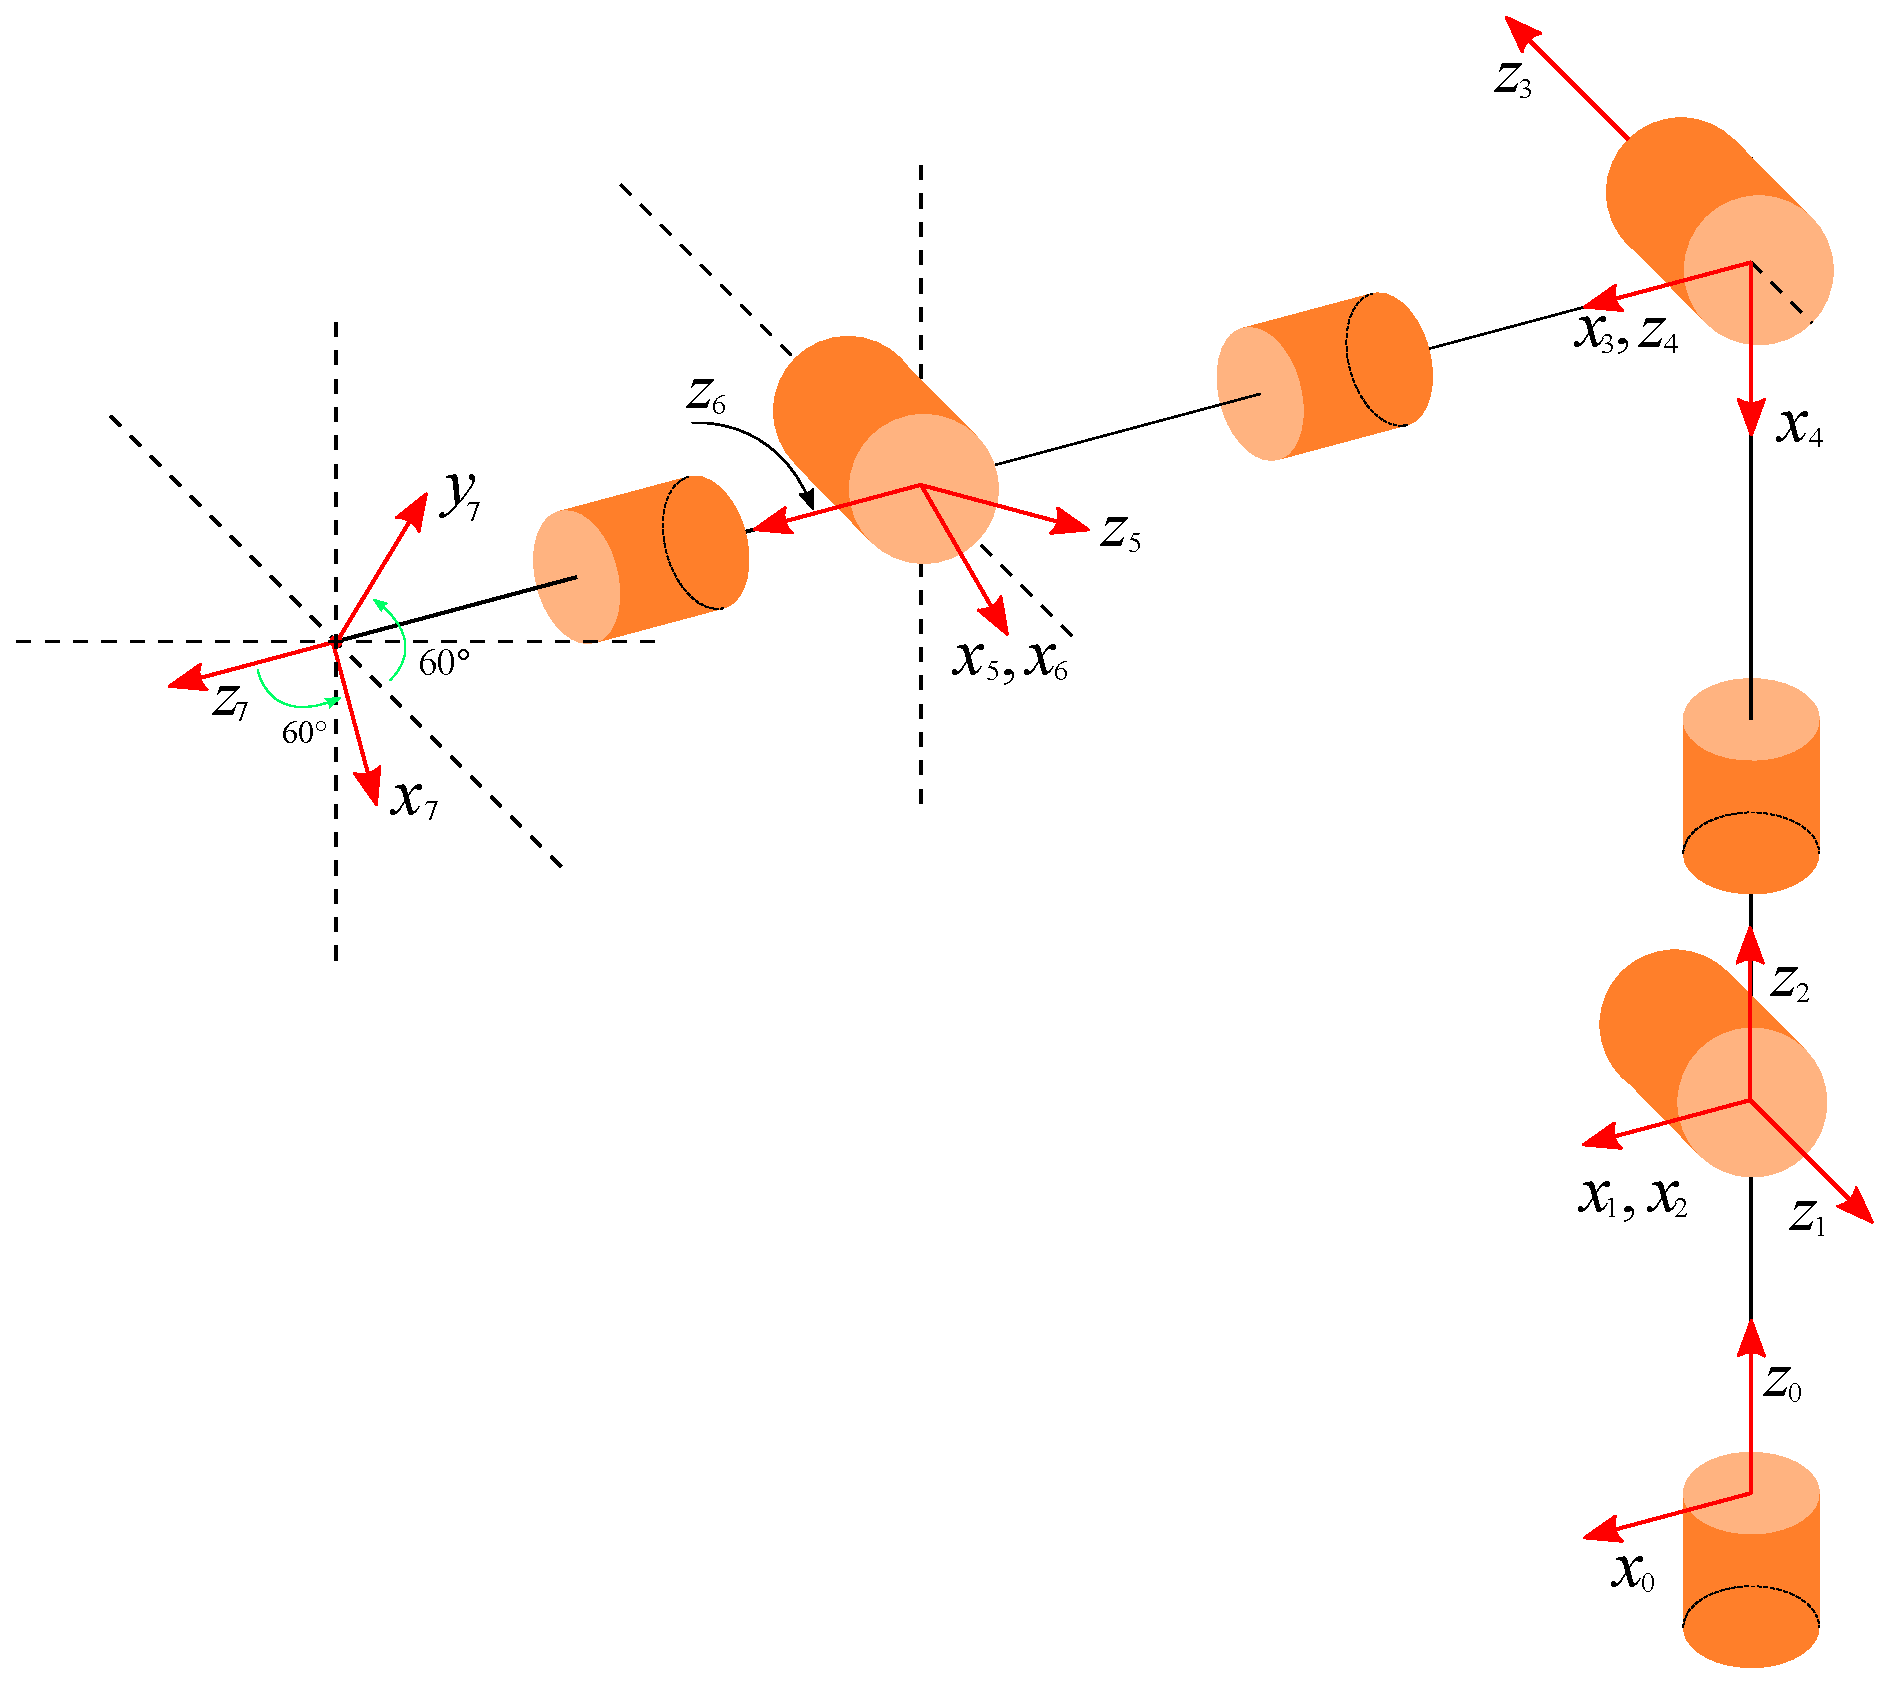
\includegraphics[width=0.9\textwidth,right]{Fig/pos_escolhida.eps}
\end{figure}
\end{columns}
\end{frame}

\begin{frame}{Comparação do software com a matriz $\mathtt{T\_}$}
\begin{columns}
\column{0.58\textwidth}
A matriz de rotação é então calculada fazendo
\begin{align*}
    R_7^0 =
    \left[ 
    \begin{array}{ccc}
        x_7 \cdot x_0 & y_7 \cdot x_0 & z_7 \cdot x_0 \\
        x_7 \cdot y_0 & y_7 \cdot y_0 & z_7 \cdot y_0 \\
        x_7 \cdot z_0 & y_7 \cdot z_0 & z_7 \cdot z_0
    \end{array}
    \right]
\end{align*}
que resulta em
\begin{align}
    R\_ &=
    \left[ 
    \begin{array}{rrr}
        0 & 0 & 1 \\
         \cos\ang{60} & \sen\ang{60} & 0 \\
        -\sen\ang{60} & \cos\ang{60} & 0
    \end{array}
    \right] \nonumber\\
    &= 
    \left[ 
    \begin{array}{rrr}
        0 & 0 & 1 \\
        \sqrt{3}/2 & 1/2 & 0 \\
        -1/2 & \sqrt{3}/2 & 0
    \end{array}
    \right]
    \label{eq:R_analise_dim}
\end{align}

\column{0.38\textwidth}
\begin{figure}
    \centering
    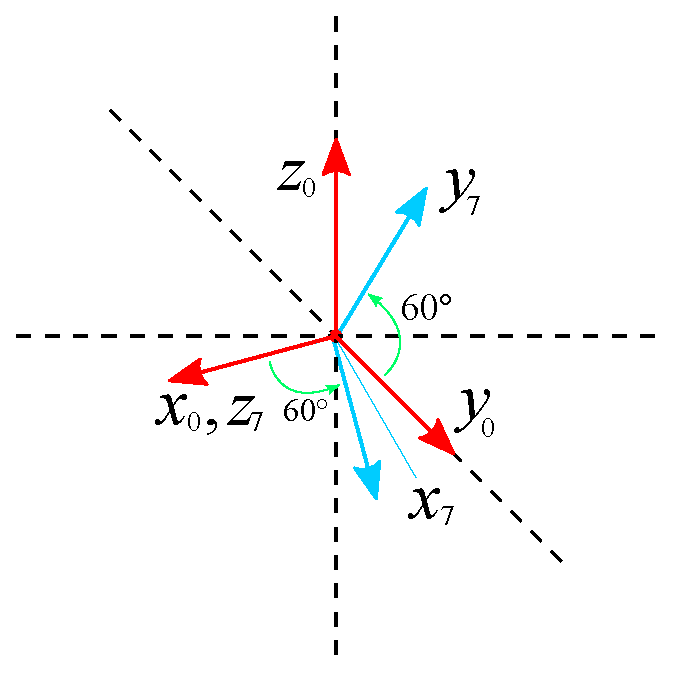
\includegraphics[width=0.8\textwidth]{Fig/zoom_pos-escolhida.eps}
    \caption{Diagrama de arames para a configuração escolhida}
    \label{fig:zoom_arames_escolhido}
\end{figure}
\end{columns}
\end{frame}

\begin{frame}{Análise dimensional da posição escolhida}
\begin{columns}
\column{0.48\textwidth}
Para a configuração escolhida ($\theta_4 = \ang{-90}$ e $\theta_5 = \ang{60}$), a matriz de transformação calculada é
\begin{align*}
    \mathtt{T\_} 
    &=
    \left[
    \begin{array}{ccc;{2pt/2pt}c}
        0 & 0 & 1 & 490 \\
        \frac{\sqrt{3}}{2} & \frac{1}{2} & 0 & 0 \\  -\frac{1}{2} & \frac{\sqrt{3}}{2} & 0 & 780 \\
        \hdashline[2pt/2pt]
        0 & 0 & 0 & 1
    \end{array}
    \right]
\end{align*}
\column{0.48\textwidth}
Comparando com a rotação \eqref{eq:R_analise_dim} obtida na análise dimensional
\begin{align*}
    R\_ = \left[ 
    \begin{array}{rrr}
        0 & 0 & 1 \\
        \sqrt{3}/2 & 1/2 & 0 \\
        -1/2 & \sqrt{3}/2 & 0
    \end{array}
    \right]
\end{align*}

Verifica-se que a orientação coincide com a submatriz de rotação e logo, o modelo de cinemática direta é validado.

\end{columns}
\end{frame}

\begin{frame}{Simulação $\mathtt{T}_\mathtt{home}$}
\begin{figure}[h]
    \centering
    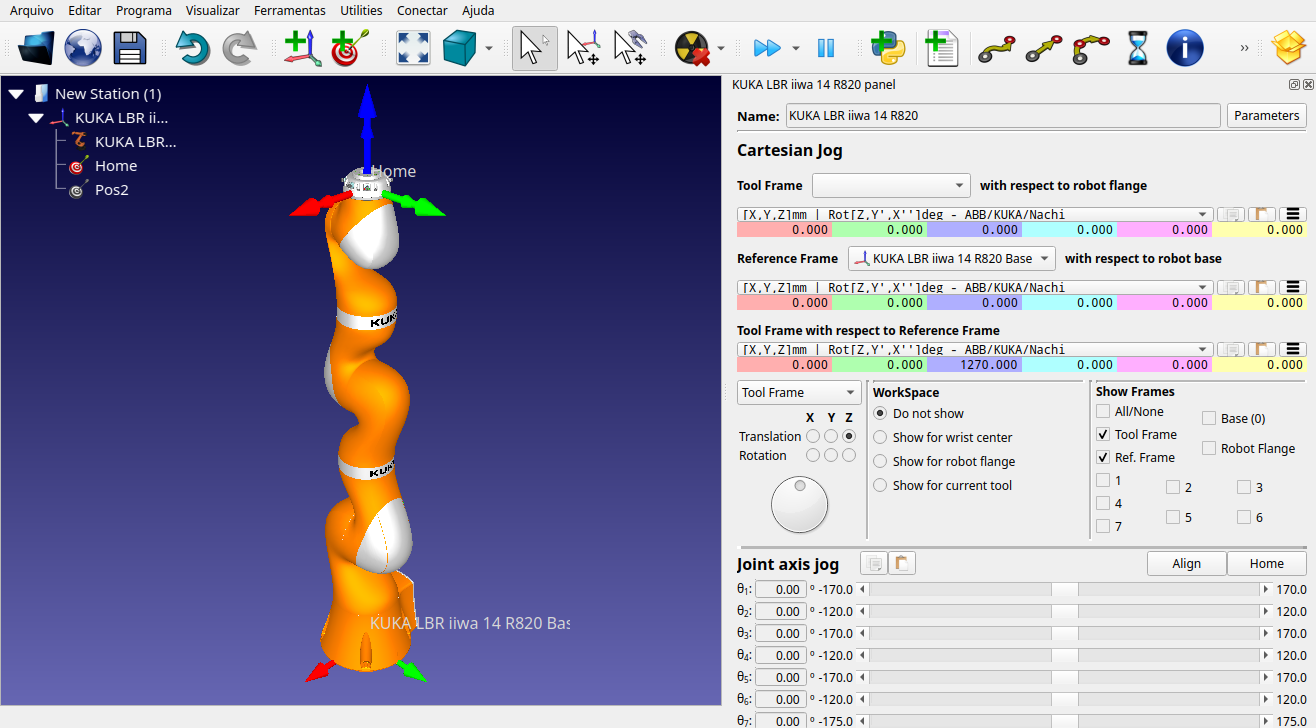
\includegraphics[width=0.75\textwidth]{Fig/home.png}
    \caption{$\mathtt{T}_\mathtt{home}$ resultante do RoboDK}
    \label{fig:Thome}
\end{figure}
\end{frame}
\begin{frame}{Simulação $\mathtt{T\_}$}
    \begin{figure}[h]
    \centering
    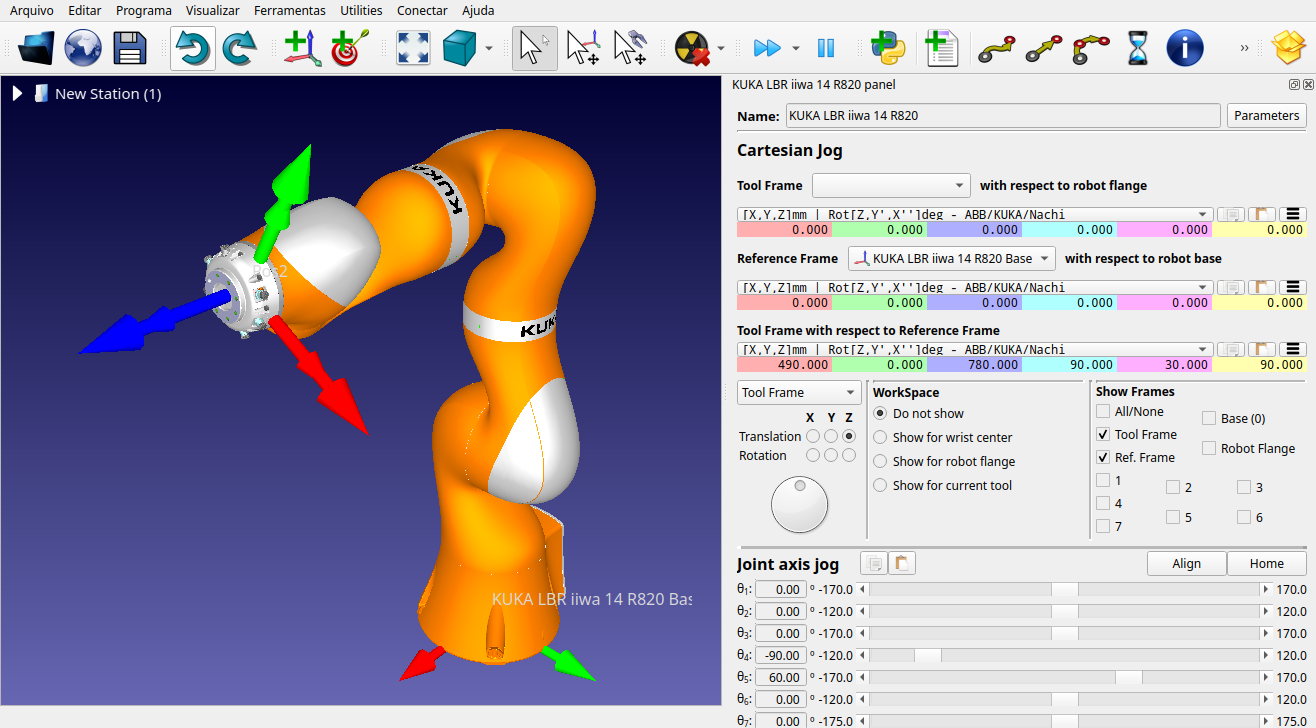
\includegraphics[width=0.75\textwidth]{Fig/escolhido.png}
    \caption{$\mathtt{T\_}$ resultante do RoboDK}
    \label{fig:Tescohido}
\end{figure}
\end{frame}

\begin{frame}{Comparação do software com a matriz $\tt T\_$}
%\begin{columns}
    %\column{0.48\textwidth}
    %No RoboDK, a pose do \textit{end-effector} é retornada com a translação nos eixos, mas a rotação em $z$, $y'$ e $x''$. Isto é, a composição de rotações no frame atual para os valores indicados.
    
    Para a configuração escolhida em $\tt T\_$, são dados
    \begin{equation*}
        R\_ = \Rot_{z,\,\ang{90}} \Rot_{y,\,\ang{30}} \Rot_{x,\,\ang{90}}
    \end{equation*}
    %\column{0.48\textwidth}
    Aplicando os valores
    \begin{align*}
    R\_ = 
        \left[ 
    \begin{array}{rrr}
        0 & -1 & 0 \\
        1 &  0 & 0 \\
        0 &  0 & 1
    \end{array}
    \right]
    \left[ 
    \begin{array}{rrr}
        \sqrt{3}/2 & 0 & 1/2 \\
        0 &  1 & 0 \\
        -1/2 &  0 & \sqrt{3}/2
    \end{array}
    \right]
    \left[ 
    \begin{array}{rrr}
        1 & 0 &  0 \\
        0 & 0 & -1 \\
        0 & 1 & 0
    \end{array}
    \right] = \left[ 
    \begin{array}{rrr}
        0 & 0 & 1 \\
        \sqrt{3}/2 & 1/2 & 0 \\
        -1/2 & \sqrt{3}/2 & 0
    \end{array}
    \right] \label{eq:R_robodk}
    \end{align*}
    cuja comparação com $\mathtt{T\_}$ valida novamente a modelagem
    \begin{align*}
    \mathtt{T\_} 
    &=
    \left[
    \begin{array}{ccc;{2pt/2pt}c}
        0 & 0 & 1 & 490 \\
        \frac{\sqrt{3}}{2} & \frac{1}{2} & 0 & 0 \\  -\frac{1}{2} & \frac{\sqrt{3}}{2} & 0 & 780 \\
        \hdashline[2pt/2pt]
        0 & 0 & 0 & 1
    \end{array}
    \right]
\end{align*}
%\end{columns}
\end{frame}

\begin{frame}{Agradecimentos}
    \begin{figure}[h]
        \centering
        
\includegraphics[width=5cm]{thank-you.eps}
    \end{figure}
\end{frame}
%---------------------------------------------------------


%---------------------------------------------------------



\end{document}